\documentclass[a4paper,twoside,11pt]{report} %openright
\newcommand{\documenttype}{Bachelor project}
\newcommand{\thesistitle}{SBML Converter for ERODE}
\newcommand{\thesissubtitle}{}

\newcommand{\thesisauthor}{Björn Wilting} % Your name :) 
\newcommand{\studentnumber}{s184214}
\newcommand{\thedate}{July 26th, 2021} % For example "June, 2019"

\newcommand{\department}{DTU Compute}
\newcommand{\departmentdescriber}{Department of Applied Mathematics and Computer Science}
\newcommand{\addressI}{Richard Petersens Plads, Building 324}
\newcommand{\addressII}{2800 Kgs. Lyngby}
\newcommand{\departmentwebsite}{www.compute.dtu.dk}

%\usepackage{microtype}      % better looking text
%\usepackage[utf8]{inputenc}
\usepackage{fontspec}       % Package for custom fonts
\usepackage[]{geometry}     % Package for changing page margins (before fancyhdr) 
\usepackage{fancyhdr}       % Package to change header and footer
\usepackage{parskip}        % Package to tweak paragraph skipping (instead of indents a small skip is added after every paragraph)
\usepackage{titlesec}
\usepackage{tikz}           % Package for drawing
\usepackage{pgfplots}       % Package for creating graphs and charts
\usepackage{xcolor}         % Package for defining DTU colours to be used
\usepackage{amsmath}        % For aligning equations among other
\usepackage{siunitx}        % SI units
\usepackage{listings}       % Package for inserting code, (before cleveref)
\PassOptionsToPackage{hyphens}{url} % Ability to line break urls at hyphens
\usepackage{hyperref}       % Package for cross referencing (also loads url package)
\usepackage{cleveref}       % improved cross referencing
\usepackage{textcomp}       % \textdegree = °C and other useful symbols
\usepackage[english]{babel} % localisation 
\usepackage{caption}        % better captions
\usepackage{subcaption}     % for subfigures
\usepackage{csquotes}       % For biblatex with babel
\usepackage[backend=biber,style=authoryear,sorting=none]{biblatex} % Package for bibliography (citing)
\bibliography{bibliography.bib}
\usepackage{tabularx}       % for ability to adjust column spacing in tabular better
\usepackage{booktabs}       % for better tables
\usepackage{float}          % floating figures in correct places
\usepackage{calc}           % Adds ability for latex to calculate (3pt+2pt) 
\usepackage[printwatermark=false]{xwatermark} % Package for wartermark. Toggle printwatermark true or false to include or remove the watermark
\usepackage{blindtext}

% Colours! 
\newcommand{\targetcolourmodel}{cmyk} % rgb for a digital version, cmyk for a printed version. Only use lowercase
\selectcolormodel{\targetcolourmodel}

% Define colours from https://www.designguide.dtu.dk/
\definecolor{dtured}    {rgb/cmyk}{0.6,0,0 / 0,0.91,0.72,0.23}
\definecolor{blue}      {rgb/cmyk}{0.1843,0.2431,0.9176 / 0.88,0.76,0,0}
\definecolor{brightgreen}{rgb/cmyk}{0.1216,0.8157,0.5098 / 0.69,0,0.66,0}
\definecolor{navyblue}  {rgb/cmyk}{0.0118,0.0588,0.3098 / 1,0.9,0,0.6}
\definecolor{yellow}    {rgb/cmyk}{0.9647,0.8157,0.3019 / 0.05,0.17,0.82,0}
\definecolor{orange}    {rgb/cmyk}{0.9882,0.4627,0.2039 / 0,0.65,0.86,0}
\definecolor{pink}      {rgb/cmyk}{0.9686,0.7333,0.6941 / 0,0.35,0.26,0}
\definecolor{grey}      {rgb/cmyk}{0.8549,0.8549,0.8549 / 0,0,0,0.2}
\definecolor{red}       {rgb/cmyk}{0.9098,0.2471,0.2824 / 0,0.86,0.65,0}
\definecolor{green}     {rgb/cmyk}{0,0.5333,0.2078 / 0.89,0.05,1,0.17}
\definecolor{purple}    {rgb/cmyk}{0.4745,0.1373,0.5569 / 0.67,0.96,0,0}

\newcommand{\dtulogocolour}{white} % Colour of the DTU logo: white, black or dtured
\newcommand{\frontpagetextcolour}{white} % front page text colour: white or black
\colorlet{frontbackcolor}{blue} % Set the background colour of the front- and back page. Choose the colour so it matches the main colour of front page picture

% DTU colours for diagrams
% You might want to make the front/back page background colour the first colour in the plot cycle list.
\pgfplotscreateplotcyclelist{DTU}{%
dtured,         fill=dtured,        \\%
blue,           fill=blue,          \\%
brightgreen,    fill=brightgreen    \\%
navyblue,       fill=navyblue       \\%
yellow,         fill=yellow         \\%
orange,         fill=orange         \\%
grey,           fill=grey           \\%
red,            fill=red            \\%
green,          fill=green          \\%
purple,         fill=purple         \\%
}


% Font
% There is no corporate serif font in the DTU design guide. The DTU design team has proposed to use Neo Sans for headings - and Arial for the body text.
% To change heading font to NeoSans Pro please upload both NeoSansPro-Regular.otf and NeoSansPro-Medium.otf to the root directory.
\setmainfont{Arial}
\renewcommand\thepart{Part \Roman{part}}
\IfFontExistsTF{NeoSansPro-Medium.otf}
{ %If True set headings to NeoSans Pro
\newfontface\NeoSansProReg{NeoSansPro-Regular.otf}
\newfontface\NeoSansProMed{NeoSansPro-Medium.otf}
\titleformat{\part}[display]{\NeoSansProMed \huge \centering}{\NeoSansProMed \Huge \thepart}{1em}{\thispagestyle{empty}}{}
\titleformat{\chapter}{\NeoSansProMed\huge}{\thechapter}{1em}{\raggedright}
\titleformat{\section}{\NeoSansProMed\Large}{\thesection}{1em}{\raggedright}
\titleformat{\subsection}{\NeoSansProMed\large}{\thesubsection}{1em}{\raggedright}
\titleformat{\subsubsection}{\NeoSansProMed\normalsize}{\thesubsubsection}{1em}{\raggedright}
\newcommand\TitleFont[1]{{\NeoSansProMed #1}}
\newcommand\titlefont[1]{{\NeoSansProReg #1}}
}
{ % If false
\titleformat{\part}[display]{\bfseries\huge \centering}{\bfseries\Huge \thepart}{1em}{\thispagestyle{empty}}{}
\titleformat{\chapter}{\bfseries\huge}{\thechapter}{1em}{\raggedright}
\titleformat{\section}{\bfseries\Large}{\thesection}{1em}{\raggedright}
\titleformat{\subsection}{\bfseries\large}{\thesubsection}{1em}{\raggedright}
\titleformat{\subsubsection}{\bfseries\normalsize}{\thesubsubsection}{1em}{\raggedright}
\newcommand\TitleFont[1]{{\bfseries #1}}
\newcommand\titlefont[1]{{#1}}
}
\urlstyle{sf}
%\def\UrlFont{\NeoSansProReg}


% If you wish to use the pdflatex compiler, sans-serif Helvetica can be used as a replacement for Arial. In this way you will be able to use the microtype package. Remember to add \usepackage[utf8]{inputenc} and disable the fontspec package. 
%\newcommand\TitleFont[1]{{\bfseries #1}}
%\newcommand\titlefont[1]{{#1}}
%\fontfamily{qhv}\selectfont
%\renewcommand{\familydefault}{\sfdefault}


% Watermark for confidential or draft (or anything else)
%\sffamily % set the correct font for the watermark
\newsavebox\mybox
\savebox\mybox{\tikz[color=grey,opacity=0.5]\node{Template};}

\newwatermark*[
  oddpages,
  angle=60,
  scale=12,
  %fontfamily=qhv,
  xpos=-40,
  ypos=30,
]{\usebox\mybox}

\newwatermark*[
  evenpages,
  angle=60,
  scale=12,
  %fontfamily=qhv,
  xpos=-50,
  ypos=30,
]{\usebox\mybox}


% Table of contents (TOC) and numbering of headings
\setcounter{tocdepth}{1}    % Depth of table of content: sub sections will not be included in table of contents
\setcounter{secnumdepth}{2} % Depth of section numbering: sub sub sections are not numbered

\makeatletter % Reset chapter numbering for each part
\@addtoreset{chapter}{part}
\makeatother  

% Spacing of titles and captions
\titlespacing\chapter{0pt}{0pt plus 4pt minus 2pt}{4pt plus 2pt minus 2pt}
\titlespacing\section{0pt}{12pt plus 3pt minus 3pt}{2pt plus 1pt minus 1pt}
\titlespacing\subsection{0pt}{8pt plus 2pt minus 2pt}{0pt plus 1pt minus 1pt}
\titlespacing\subsubsection{0pt}{4pt plus 1pt minus 1pt}{-2pt plus 1pt minus 1pt}
\captionsetup{belowskip=\parskip,aboveskip=4pt plus 1pt minus 1pt}

% Setup header and footer
\fancypagestyle{main}{% All normal pages
    \fancyhead{}
    \fancyfoot{}
    \renewcommand{\headrulewidth}{0pt}
    \fancyfoot[LE,RO]{\footnotesize \thepage}
    \fancyfoot[RE,LO]{\footnotesize \thesistitle} % - \rightmark
    \fancyhfoffset[E,O]{0pt}
}
\fancypagestyle{plain}{% Chapter pages
    \fancyhead{}
    \fancyfoot{}
    \renewcommand{\headrulewidth}{0pt}
    \fancyfoot[LE,RO]{\footnotesize \thepage}
    \fancyfoot[RE,LO]{\footnotesize \thesistitle} % - \leftmark
    \fancyhfoffset[E,O]{0pt}
}


% Setup for diagrams and graphs (tikz pictures) 
\usetikzlibrary{spy}    % For magnifying anything within a tikzpicture, see the line graph
\usepgfplotslibrary{statistics} % Package for the boxplot
\pgfplotsset{ % Setup for diagrams
compat=newest,
major x grid style={line width=0.5pt,draw=grey},
major y grid style={line width=0.5pt,draw=grey},
legend style={at={(0.5,-0.1)}, anchor=north,fill=none,draw=none,legend columns=-1,/tikz/every even column/.append style={column sep=10pt}},
axis line style={draw=none},
tick style={draw=none},
every axis/.append style={ultra thick},
tick label style={/pgf/number format/assume math mode}, % To apply main font to tick labels (numbers on the axis)
}
\tikzset{every mark/.append style={scale=1.5}}


% Hypersetup
\hypersetup{
    pdfauthor={\thesisauthor},
    pdftitle={\thesistitle},
    pdfsubject={\thesissubtitle},
    pdfdisplaydoctitle,
    bookmarksnumbered=true,
    bookmarksopen,
    breaklinks,
    linktoc=all,
    plainpages=false,
    unicode=true,
    colorlinks=false,
    hidelinks,                        % Do not show boxes or coloured links.
}


% Listings setup
\lstset{
    basicstyle=\footnotesize\ttfamily,% the size of the fonts that are used for the code
    commentstyle=\color{green},       % comment style
    keywordstyle=\bfseries\ttfamily\color{blue}, % keyword style
    numberstyle=\sffamily\tiny\color{grey}, % the style that is used for the line-numbers
    stringstyle=\color{purple},       % string literal style
    rulecolor=\color{grey},           % if not set, the frame-color may be changed on line-breaks within not-black text (e.g. comments (green here))
    breakatwhitespace=false,          % sets if automatic breaks should only happen at whitespace
    breaklines=true,                  % sets automatic line breaking
    captionpos=b,                     % sets the caption-position to bottom
    deletekeywords={},                % if you want to delete keywords from the given language
    escapeinside={\%*}{*)},           % if you want to add LaTeX within your code
    frame=single,                     % adds a frame around the code
    xleftmargin=4pt, 
    morekeywords={*,...},             % if you want to add more keywords to the set
    numbers=left,                     % where to put the line-numbers; possible values are (none, left, right)
    numbersep=10pt,                   % how far the line-numbers are from the code
    showspaces=false,                 % show spaces everywhere adding particular underscores; it overrides 'showstringspaces'
    showstringspaces=false,           % underline spaces within strings only
    showtabs=false,                   % show tabs within strings adding particular underscores
    stepnumber=1,                     % the step between two line-numbers. If it's 1, each line will be numbered
    tabsize=2,                        % sets default tabsize to 2 spaces
    title=\lstname,                   % show the filename of files included with \lstinputlisting; also try caption instead of title
}

% Signature field
\newlength{\myl}
\newcommand{\namesigdatehrule}[1]{\par\tikz \draw [black, densely dotted, very thick] (0.04,0) -- (#1,0);\par}
\newcommand{\namesigdate}[2][]{%
\settowidth{\myl}{#2}
\setlength{\myl}{\myl+10pt}
\begin{minipage}{\myl}%
\begin{center}
    #2  % Insert name from the command eg. \namesigdate{\authorname}
    \vspace{1.5cm} % Spacing between name and signature line 
    \namesigdatehrule{\myl}\smallskip % Signature line and a small skip
    \small \textit{Signature} % Text under the signature line "Signature"
    \vspace{1.0cm} % Spacing between "Signature" and the date line
    \namesigdatehrule{\myl}\smallskip % Date line and a small skip
    \small \textit{Date} % Text under date line "Date" 
\end{center}
\end{minipage}
}

% For the back page: cleartoleftpage
\newcommand*\cleartoleftpage{%
  \clearpage
  \ifodd\value{page}\hbox{}\newpage\fi
}


\usepackage{hyperref}
\usepackage{pifont}
\usepackage{subcaption}


\hypersetup{
    colorlinks=true,
    linkcolor=blue,
    filecolor=magenta,      
    urlcolor=cyan,
}


\title{SBML Converter for ERODE}
\author{s184214 }
\date{April 2021}

%%%%%%%%%%%%%%%%%%%%%%%%5
%%%%%%%%%%%%%%%%%%%%%%%%%GEORGIOS COMMANDS

\usepackage[utf8]{inputenc}
\usepackage{blindtext}
\usepackage[utf8]{inputenc}
\usepackage[english]{babel}
\usepackage{float}
\usepackage{caption}
%\usepackage{subcaption}
\usepackage{hyperref}
\usepackage[section]{placeins}
\usepackage{amsthm}
\usepackage{amsmath}
\usepackage{tikz}
\usepackage{verbatim}



\theoremstyle{remark}
\newtheorem*{remark}{Remark}

\usepackage{amssymb}%Andrea: for \nexists
\usepackage{verbatim}
\usepackage{xargs}
\usepackage{amsfonts}
\usepackage{tikz}

\usepackage{enumitem}
\usepackage{lipsum}

\newlist{mylistenv}{enumerate}{3}
\newenvironment{mylist}[1]{%
	\setlist[mylistenv]{label=#1\arabic{mylistenvi}.,ref=#1\arabic{mylistenvi}}%
	\setlist[mylistenv,2]{label=#1\arabic{mylistenvi}.\arabic{mylistenvii}.,ref=#1\arabic{mylistenvi}.\arabic{mylistenvii}}%
	 \setlist[mylistenv,3]{label=#1\arabic{mylistenvi}.\arabic{mylistenvii}.\arabic{mylistenviii}.,ref=#1\arabic{mylistenvi}.\arabic{mylistenvii}.\arabic{mylistenviii}}%
	\renewenvironment{mylist}{\begin{mylistenv}}{\end{mylistenv}}
	\begin{mylistenv}%
	}{%
	\end{mylistenv}%
}
\usepackage{array}

\usepackage{amsthm}
\usepackage{amsmath}
\usepackage{tikz}


%%%%%%%%%%%%%%%%%%%% GHERKIN CODE COLORING %%%%%%%%%%%%%%%%%%%%%%%%%%
\usepackage{listings,xcolor}

\definecolor{words}{rgb}{0.80,0.40,0}
\definecolor{bluekeywords}{rgb}{0.13,0.13,1}
\definecolor{greencomments}{rgb}{0,0.5,0}
\definecolor{turqusnumbers}{rgb}{0.17,0.57,0.69}
\definecolor{redstrings}{rgb}{0.5,0,0}
\definecolor{xmlDefault}{rgb}{0.8,0,0.13}
\definecolor{xmlString}{rgb}{0.33,0.50,0.00}
\definecolor{greenTic}{rgb}{0.1,0.6,0}

\lstdefinelanguage{Gherkin} {
    basicstyle=\ttfamily,
    columns=fullflexible,
    showstringspaces=false,
    commentstyle=\color{gray}\upshape,
    morestring=[b]",
    morekeywords={Background, Feature, Scenario, Given, When, Then, And},
    keywordstyle=\color{words},
    sensitive=true,
    morecomment=[l][\color{greencomments}]{\#},
    morestring=[b]",
    stringstyle=\color{bluekeywords}
    }
%%%%%%%%%%%%%%%%%%%%%%%%%%%%%%%%%%%%%%%%%%%%%%%%%%
%%%%%%%%%%%%%%%%%% XML code coloring %%%%%%%%%%%%%%%%%
\lstdefinelanguage{SBML} {
      basicstyle=\ttfamily,
      columns=fullflexible,
      showstringspaces=false,
      commentstyle=\color{gray}\upshape,
      morestring=[b]",
      moredelim=[s][\bfseries\color{xmlDefault}]{<}{\ },
      moredelim=[s][\bfseries\color{xmlDefault}]{</}{>},
      moredelim=[l][\bfseries\color{xmlDefault}]{/>},
      moredelim=[l][\bfseries\color{xmlDefault}]{>},
      morecomment=[s]{<?}{?>},
      morecomment=[s]{<!--}{-->},
      stringstyle=\color{xmlString},
      identifierstyle=\color{xmlDefault},
      keywordstyle=\color{orange},
      morekeywords={xmlns,version,type, level, required, id, name, compartment, maxLevel,
      initialLevel, constant, qualitativeSpecies, resultLevel,}
    }
%%%%%%%%%%%%%%%%%%%%%%%%%%%%%%%%%%%%%%%%%%%%%%%%%%%%%%%
%%%%%%%%%%%%%%%%%%%% Java Syntax Highlighting %%%%%%%%%%%
\lstset {
    language=Java,
    basicstyle=\ttfamily,
    columns=fullflexible,
    showstringspaces=false,
    commentstyle=\color{gray}\upshape,
    morestring=[b]",
    keywordstyle=\color{blue},
    sensitive=true,
    commentstyle=\color{greencomments},
    stringstyle=\color{bluekeywords}
}

%%%%%%%%%%%%%%% ERODE %%%%%%%%%%%%%%%%%%%%%%%%%%%%
\lstdefinelanguage{ERODE} {
      basicstyle=\ttfamily,
      columns=fullflexible,
      showstringspaces=false,
      commentstyle=\color{gray}\upshape,
      keywordstyle=\color{xmlDefault},
      morekeywords={begin, Boolean, network, init, end, update, functions}
    }

%%%%%%%%%%%%%%%%%%%% CHECKLIST %%%%%%%%%%%%%%%%%%%%%%%
\newcommand{\gcheck}[0]{\color{greenTic}\ding{51}}
\newcommand{\xcheck}[0]{\color{red}\ding{55}}

\theoremstyle{remark}



% Comments and notes
\usepackage{todonotes}
\newcommandx{\todos}[2][1=]{\todo[inline,caption={},linecolor=red,backgroundcolor=red!25,bordercolor=red,#1]{\textbf{TODO: }#2}}
\newcommandx{\commentGeorgios}[2][1=]{\todo[inline,caption={},linecolor=red,backgroundcolor=red!25,bordercolor=red,#1]{\small#2\textbf{\\-- Georgios}}\xspace}
\newcommandx{\commentAlberto}[2][1=]{\todo[inline,caption={},linecolor=cyan,backgroundcolor=cyan!25,bordercolor=cyan,#1]{\small#2\textbf{\\-- Alberto}}\xspace}
\newcommandx{\commentAndrea}[2][1=]{\todo[inline,caption={},linecolor=purple,backgroundcolor=purple!25,bordercolor=purple,#1]{\small#2\textbf{\\-- Andrea}}\xspace}
\newcommand{\coma}[1]{{\color{red}[AV:#1]}}
\newcommand{\comg}[1]{{\color{blue}[G:#1]}}
\newcommand{\comal}[1]{{\color{purple}\hl{[AL:#1]}}}
\newcommand{\comax}[1]{{\color{purple}[Max: #1]}}
\newcommand{\mv}[1]{{\color{red}#1}}


%%%%%%%%%%%%%%%%%%%%%%%%%%%%%%%%%
%%%%%%%%%%%%%%%%%%%%%%%%%%%%%%%%%%%%%%
%%%%%%%%%%%%%%% END OF GEORGIOS COMMANDS

\begin{document}

\pagenumbering{roman}
\title{\thesistitle} 
\author{\thesisauthor} 
\date{\thedate} 

\begin{titlepage}

\newgeometry{left=11mm,right=11mm,top=50mm,bottom=0pt}
\pagecolor{frontbackcolor}
\color{\frontpagetextcolour}

{ % Thesis title (to change see Setup/Settings.tex) 
\Huge
\begin{tabular}{p{\linewidth}}
\TitleFont{\thesistitle}   \\ 
\TitleFont{\thesissubtitle} \bigskip \\ 
\titlefont{\documenttype}
\end{tabular}
}

% DTU department (to change see Setup/Settings.tex) 
\begin{tikzpicture}[remember picture,overlay]
\node[anchor=north east, 
      xshift=-10mm, 
      yshift=-12mm] 
      at (current page.north east) 
      {
        \color{\frontpagetextcolour}
        \begin{tabular}{r} 
        \textbf{\department} \\ 
        \departmentdescriber
        \end{tabular}
      }; 
\end{tikzpicture}

% DTU logo
\begin{tikzpicture}[remember picture,overlay]
\node[anchor=north west, 
      xshift=8.9mm, 
      yshift=-8.3mm] 
     at (current page.north west) 
     {\includegraphics[width=14.75mm,keepaspectratio]{Pictures/Logos/\dtulogocolour_\targetcolourmodel.pdf}}; 
\end{tikzpicture}

% Cover photo
\begin{tikzpicture}[remember picture,overlay]
\node[anchor=south, % anchor is bottom of picture
      xshift=0pt, 
      yshift=-2.9mm] % shifting picture to actually be at the bottom of the page
     at (current page.south) % placement at bottom of the page
     {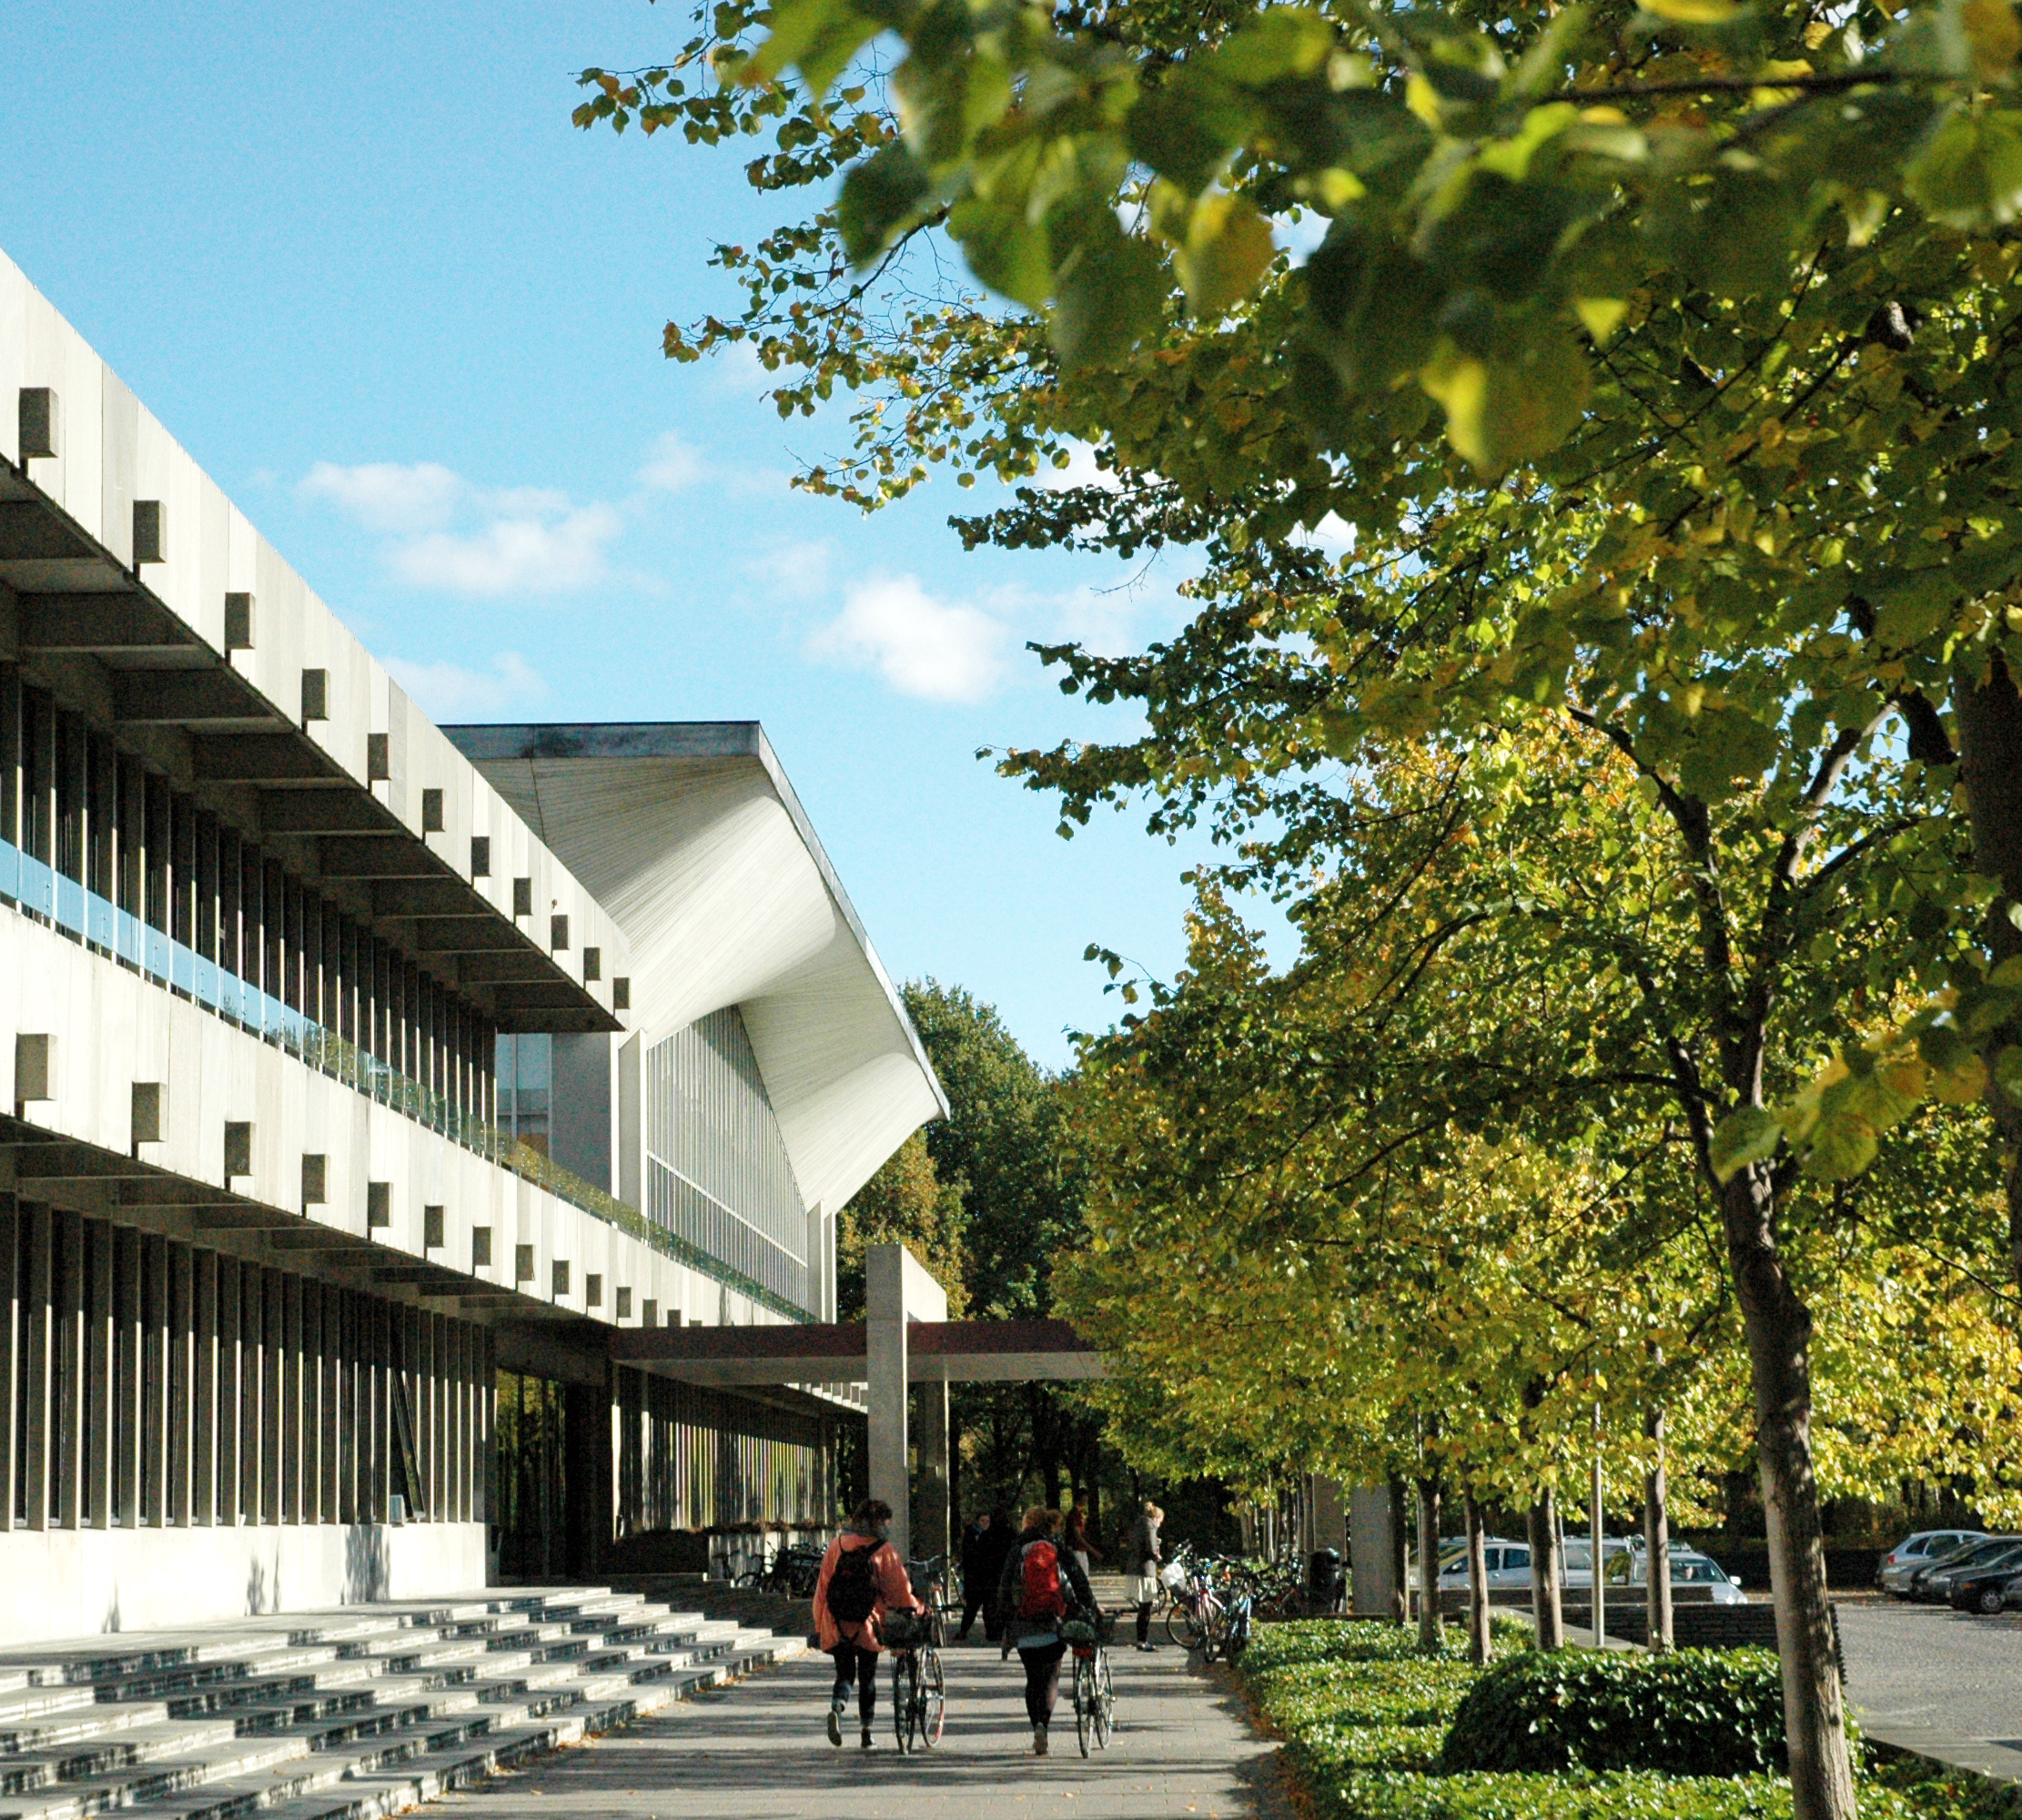
\includegraphics[height=18.9cm,keepaspectratio]{Pictures/DTU_stock_photo.jpg}};
\end{tikzpicture}




\end{titlepage}

\pagecolor{white}
\newgeometry{top=2.81cm, bottom=2.75cm, outer=2.5cm, inner=3.5cm}
\pagestyle{empty}
\thispagestyle{empty}
\setcounter{page}{1}
\vspace*{\fill}

\textbf{\thesistitle} \newline
\thesissubtitle

\smallskip

\documenttype \newline
\thedate

\smallskip

By \newline
\thesisauthor~\studentnumber

\bigskip

\begin{tabularx}{\textwidth}{@{}lX@{}}
    Supervisors: & Andrea Vandin, Georgios Agyris and Alberto Lluch Lafuente \\
    \\
    Copyright: & Reproduction of this publication in whole or in part must include the customary bibliographic citation, including author attribution, report title, etc. \\
    Cover photo: & Vibeke Hempler, 2012 \\
    Published by: & DTU, \departmentdescriber, \addressI, \addressII ~Denmark  \\
     & \url{\departmentwebsite} \\
    %ISSN: & [0000-0000] (electronic version) \\
    %ISBN: & [000-00-0000-000-0] (electronic version) \\
    %& \\
    %ISSN: & [0000-0000] (printed version) \\
    %ISBN: & [000-00-0000-000-0] (printed version)
\end{tabularx}



\clearpage 
\pagestyle{main}
%\section*{Approval}
\addcontentsline{toc}{section}{Preface}
This thesis has been prepared over six months at the Section for Indoor Climate, Department of Civil Engineering, at the Technical University of Denmark, DTU, in partial fulfilment for the degree Master of Science in Engineering, MSc Eng. 

It is assumed that the reader has a basic knowledge in the areas of statistics. 

\vfill

\begin{center}
\namesigdate{\thesisauthor~-~\studentnumber}
\end{center}

\vfill


%\clearpage 
\section*{Abstract}
\addcontentsline{toc}{section}{Abstract}

ERODE is tool to analyse various types of models using a special language format developed for this purpose. SBML is a widely used XML-based format that can represent a vast amount of different biological models. The aim of this project is to develop a converter between ERODE and SBML-qual, an SBML-extension used to represent the model types that are supported by ERODE. To develop such a converter, the project begins with an analysis of both formats and the conversion requirement. The obtained knowledge is then used to design and implement the converter. During the entire development process, the project is being tested extensively to ensure a correct conversion.






\clearpage 
%\section*{Acknowledgements}
\addcontentsline{toc}{section}{Acknowledgements}
\textbf{\thesisauthor}, MSc Civil Engineering, DTU \newline
Creator of this thesis template.

\textbf{[Name]}, [Title], [affiliation] \newline
[text]

\textbf{[Name]}, [Title], [affiliation] \newline
[text]


%\cleardoublepage 
\tableofcontents
\clearpage

%%%%%%%%%%%%%%%%%%%%%%%%%%%%%%%%%%%%%%%%%%%%%%%%%%%%%%%
\pagenumbering{arabic}
\chapter{Introduction}

Mathematical models constitute the study basis of real world systems from various scientific domains like biology, physics and computer science. The complexity of systems leads to large mathematical models with many variables and parameters which hinders our capability to manipulate them and explore their properties. \href{https://www.erode.eu/}{ERODE} (\cite{erode}) is a tool to analyze, simulate and minimize 
many types of models like ordinary differential equations, chemical reaction networks, and Boolean Networks (BNs).  Since ERODE uses its own language to execute these tasks, it is often necessary to translate representations of such systems into the format of ERODE.   

Boolean Networks (BNs) constitute an established qualitative
modelling approach for biological systems. Currently, ERODE has only limited support for BNs, wherein variables take values in the Boolean domain (\{0,1\}). However, support is under development for multi-valued networks (MNs), wherein variables take values in some bounded integer domain e.g. \{0,1,2\}. SBML (Systems Biology Markup Language) is the most common representation format for biological systems, and, particularly, SBML-qual is an extension of SBML designed for the representation of BNs and MNs. 

The goal of this project is to create a converter that can translate between the formats SBML-qual and ERODE. The converter tool is developed in Java and is based on the JSBML-library (\cite{sbmlteam_2020}), a library providing framework to parse SBML files. Given that ERODE is written in Java as well, the converter is developed as a plugin, that can be integrated into ERODE and as a standalone application.


%Additionally, the converter should also be able to translate ERODE output data back into the form of  SBML. \comg{The goal of this project is to create an importer that can translate SBML-qual into the format of ERODE and vice versa.} The converter tool should be created in Java and be based on the JSBML library, a library providing framework to parse SBML files.\comg{The converter comes as a stand-alone application written in Java and based on JSBML- a library that provides a framework to parse SBML files.} The importer should come as a stand-alone application. However, given that ERODE is written in Java as well, the importer might also be fully integrated within ERODE. \comg{Since ERODE is a java application, it will be able to fully integrate the importer.}

\section{Report structure}

The report is organized as follows: Section 2 presents project's objectives and the project management. Section 3 introduces the various tools and technologies used to complete the project. In section 4, a thorough analysis of both the SBML-qual and ERODE formats is given. This analysis is then used to explain how to convert between the two formats. Section 5 explains the system architecture that was designed for this conversion process. The report continues with the implementation of this system in section 6. Particularly, this section focuses on the implementation of the individual converter components and the conversion of mathematical expressions. Section 7 explains how testing was used to ensure a correct conversion, after which a demonstration of the conversion process is given with a small demo application in section 8. In section 9, a few ideas of possible extensions or optimizations to the final converter are given, before the report is wrapped up by a conclusion in section 10.

%Section 3, analyze the problem
%Section 4, how to design the converter
%Section 5, Implementation
%Section 6, Testing
%Section 7, 
%Tools & Technologies - present tools used during this project
%Analysis - Analyze and explain the various tools
%Design - Show the design of the program, and justify design choices
%Implementation - ???
%Testing - Show testing approach, evaluate tests?
%Evaluation - What goals were achieved? Improvements? Extensions?
%Conclusion
\clearpage 
\chapter{Project Management} \label{management}
% List project objectives
% Define project goal clearly
% - Create standalone Java program that can convert SBML files into the format of ERODE
% - The program should also be able to translate ERODE output back into SBML
% - Add support for both BNs and multi-valued networks in the converter
% - Integrate the converter into ERODE
Managing a project is just as important as working on the project itself, as is allows to direct the project towards a designated goal. For this project the first step was to divide it into several stages. For each stage, a milestone was defined, declaring what should be achieved during that stage. During the project, some of the original milestones eventually had to be abandoned, as it for example was discovered that the available tools were unable to achieve the desired result or that the amount of work required would extend far beyond the project's time frame. Specifically, the milestone to add support for the conversion of multi-valued networks (MNs) had to be abandoned, because ERODE's developers were unable to add support for MNs within the time-frame of this project.

The following list contains all milestones that were kept until the end of the project:
\begin{itemize}
    \item \textbf{Familiarize with SBML and the JSBML-library.} In order to. eventually, create a converter between SBML and ERODE, it is required to understand how biological models are represented in SBML. The same goes for the JSBML-library as it is a library used to represent SBML-models in Java.
    
    \item \textbf{Create a few small JSBML demos, that can extract data from SBML files.} These demos were used as small stepping stones, towards the construction of the converter and an opportunity to experiment with the JSBML-library.
    %\comg{the first one refers to the Qualitative modelling of the network controlling Trp biosynthesis \url{http://ginsim.org/node/50}, the second one refers to cortical area development (CAD), and the third refers to "let's find a third one"}
    \item \textbf{Create a prototype SBML converter that can generate ERODE-files from an SBML-qual input.} In this first stage, the aim was to develop a basic framework for the conversion, a proof of concept for the later stages of the converter.
    \item \textbf{Extend the prototype to support all kinds of BNs by adding support for all Boolean operators supported by SBML.} 
    
    \item \textbf{Extend the prototype to support conversion from ERODE to SBML.}
    \item \textbf{Test changes and added features during development.} This is required to ensure a correct conversion between the two models representations. By testing each newly added feature and ensuring that the previously added tests still succeeds,  this can be verified.
    
    \item \textbf{Extract the core functionality to a Java-library to support integration into other projects.} By decoupling the core functionality of the converter from its program shell, the library could be used as a plugin in other projects. As an example, the converter could be integrated into ERODE, to allow direct importing and exporting of SBML-files.
    
\end{itemize}

To achieve these milestones the project was planned, and its progress tracked, on two different levels. On project level, the milestones and a few larger tasks were  planned and monitored using a Gantt-chart to visualize the overall progression. Additionally, weekly meetings with the supervisors were used to plan and track the progress of the individual milestones.
\begin{figure}[H]
    \centering
    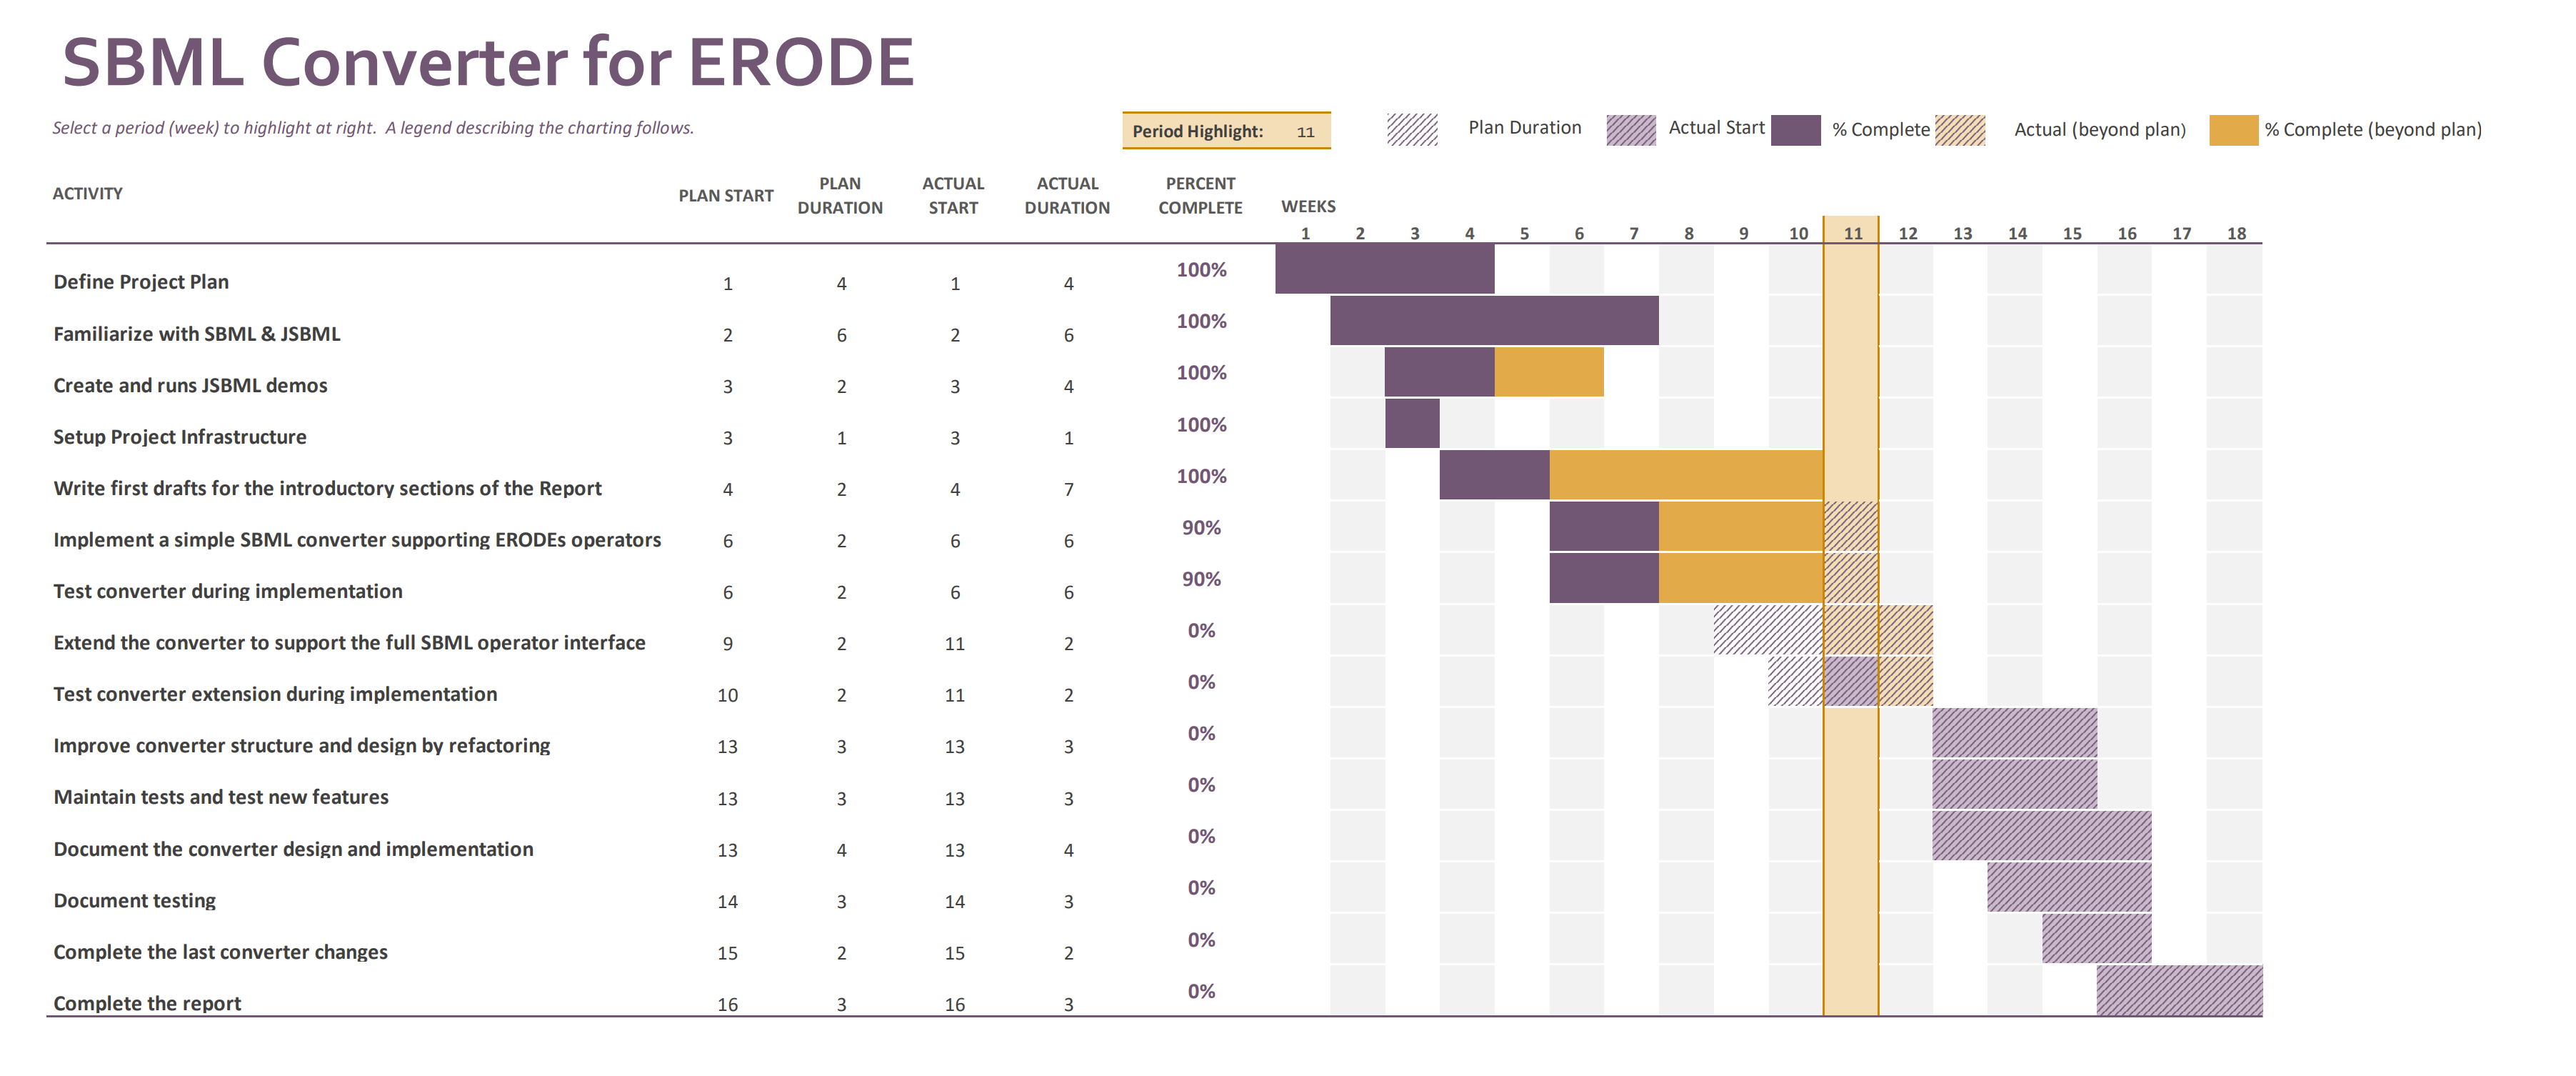
\includegraphics[scale=0.38]{Sections/Images/Project Plan.jpg}
    \caption{Gantt chart used to track the project's progress}
    \label{fig:gantt}
\end{figure}
The project code was managed using GitHub as a version control system and the Apache Maven (\cite{porter_zyl_lamy}) development tool as a code management for Java-projects (see section 3).
The \href{https://github.com/Unfunctioned/SBML-Converter-for-ERODE}{GitHub repository} can be found at \url{https://github.com/Unfunctioned/SBML-Converter-for-ERODE}.
%The next step was then to manage the required time for each milestone. This was achieved by 
%Since time is a limited resource for this project, it needs to be managed as one.\comg{?} To do so project management is required, which for this project needs to cover three different aspects.

%\begin{enumerate}
%    \item \textbf{Planning} as a means to direct the project towards its intended goal.
%    \item \textbf{Progress tracking} in order to monitor resources and adjust planning according to their changes.
%    \item \textbf{Code Management} in order to maintain a simple and efficient workflow.
%\end{enumerate}
%The planning and progress tracking of the project has been executed on two different levels. On a more abstract level the major project objectives have been planned and tracked using a Gantt-chart to give a general overview of the entire project and track its progress. On a more detailed level, weekly meetings with the supervisors have been used to plan and track the progress of the individual tasks that make up each objective on a week-to-week basis.
%\begin{comment}
%INSERT GANTTCHART HERE
%\end{comment}

%The project code has been managed using Git as a version control system (VCS) and Apache Maven to simplify the development workflow of the Java-project.

%The GitHub-repository can be found at: \verb+INSERT LINK HERE+


\begin{comment}
Project Management:
- Planning
- Code management
- Progress tracking
\end{comment}



%Present project plan with graphics
%Kanban boards for details task tracking
% - Those were later discontinued, due to giving little to no management benefit
%Apache Maven
% - Move tool section here!
\clearpage 
\chapter{Tools and Technologies}

\section{SBML \& JSBML}

%What is SBML?
    %A format to represent biological models that can be read by a machine
%What is it used for?
    %Data exchange format (language) between tools that do not share a common language
    
The Systems Biology Markup Language (SBML, \cite{hucka2018systems}) is a common XML-based format used to represent biological systems for computational modelling. The SBML format comes with multiple extensions that provide additional features, depending on the nature of the model. For example, variables may take values in the real, Boolean or multivalued domain. The different SBML extensions support several types of variables. This project focuses on SBML-qual, an extension used to represent both Boolean and multivalued networks.
%\comg{We focus on SBML-qual an extension used for BN and MN representation.}
%One of these extensions is SBML-qual, a module that can be used to represent BNs and MNs.

%It comes with an extension SBML-qual that is designed to represent both boolean and \comg{multi-valued} many-valued networks. (...)
The models represented in SBML format become available to Java using the JSBML library (\cite{sbmlteam_2020}). It is an open source pure Java API designed specifically to parse and write SBML and its extensions. When parsing an SBML-file, JSBML replicates the structure of the SBML-file using Java-objects, where each of these objects represents of the SBML-elements. Once parsing is complete, the entire structure is provided to the host program.

%What is JSBML?
    % A pure JAVA API to parse SBML files
    % platform independent
    % open source
    
%How does the JSBML library work?
%What were the first steps to learn and use the library?

\section{Apache Maven}
%What is Apache Maven?
    %Project management tool for Java projects
%What primary benefits does it provide for this project?
    %Easy build process with uniform build system, Maven handles everything from project dependencies to building, running and testing projects
    %The workflow for maven project will be same no matter the size of the project
    %Provides project information, such as unit test reports and code coverage information
    
%Check where references to - https://maven.apache.org/what-is-maven.html - are meeded
% Also - https://en.wikipedia.org/wiki/Apache_Maven
Apache Maven (\cite{porter_zyl_lamy}) is a project management tool that provides a wide range of useful features for the development of Java projects. Particularly, the tool provides uniform build system, simple dependency management framework, and unit testing capabilities.

Maven projects are built using a project object model (POM) that contains all configurations, dependencies and plugins. The POM is loaded from the \emph{pom.xml} file, and is also used to manage dependencies to external sources.
Once the developer has supplied all necessary dependency configurations to Maven, it will automatically download and install the required resources. This requires that they exist in the Maven Central Repository \cite{mavenDB}, a public database containing millions of Java-modules. In case some resources do not exist in the repository, it is however still possible to add them manually.
In addition to managing all project configurations, Maven also detects source files. This removes the need to specify, what files to use when building the project.
%\comg{a sentence should not contain more than 25 words.}

Maven is also a very useful tool, when it comes to testing projects, using unit test or similar, as the tool is capable of detecting implemented tests. This makes it possible to use Maven's interface to run tests and collect Maven generated test reports, instead of running tests manually.
%The most important features for this project being\comg{is}, the uniform build system, simple dependency management and unit test reporting with code coverage. \comg{The uniform-build system, the simple dependency management framework, and the unit test reporting with code coverage constitute some crucial features related with the project.}

%One of the great strengths of Maven is that it build process \comg{Maven's build process} is almost fully automated, as\comg{since} the developer only needs to specify build configurations. The configurations are given to Maven using the project object model (POM), which contains all project configurations for the entire project.\comg{The project object model (POM), included in Maven, contains/incorporates all required configurations for the project.} The POM is available to the developer through an XML file, which can be used by developers to configure Maven \comg{so that it fits the specific needs of their project.} to fit the specific needs of their project.

%Another important part of a project's configuration is its dependencies to external sources. Especially, when a project has many dependencies, managing the can be quite difficult.\comg{Especially, managing the dependencies is quite difficult when a project has many of them.} Using Maven, having many dependencies is not a problem. \comg{One can overcome this problem with Maven.} Once a developer has configured a dependency in the POM, Maven will automatically download the module and all of its dependencies.

%Last but not least, Maven reports on unit test results and code coverage, which makes the development of projects substantially easier, when using development processes such as Test Driven Development (TDD).

\section{Cucumber and the Gherkin language}
Cucumber Open (\cite{cucumber}) is an open source tool created to support Behaviour Driven Development (BDD), a development process that allows collaboration between programmers and non-programmers. Tests are defined used the Gherkin language, a verbose language that makes it anyone to define system tests. Once the tests are defined in \emph{feature-files (.feature format)}, the developers can use Cucumber to implement the various steps of a test scenario. Cucumber will then, map the steps definitions from the feature file to the Java test methods executing these steps. Due to this method mapping, a step definition can be reused in other scenarios requiring the same action, making it possible to assemble scenarios in a building-block-like manner.

To define a cucumber scenario, three different types of step definitions are required. The \emph{Given} step defines the initial state of the scenario. Once this state has been defined, a system action can be defined using the \emph{When} keyword for the next step definition. The code mapped to the \emph{When} statement will simulate the system action, when executing the test scenario. Finally, for a meaningful scenario it is also required to assert if the simulation ended as intended. For this, \emph{Then} statement can be defined to define how the expected end state.

The advantage of using Cucumber instead of e.g. regular unit tests is that the building-block-like structure of cucumber scenarios allows to minimize the test code. Often used steps only need to be implemented once, because each step can be executed independently. Another advantage is that the verbose test scenarios also can be used as system documentation that does not require the ability to read code. Finally, also due to the verbose nature of the scenario definitions, the choice of words for these definitions can be selected to fit a certain type of reader. For example, if the developers are the only people reading the test documentation, some technical language may be included. On the other hand, if the intended reader is  a manager or customer without the technical know-how, technical terms should generally be avoided.

\begin{lstlisting}[language=Gherkin]
    #Some cucumber scenario examples written in Gherkin
    Feature: Converting SBML files
    
        Scenario: Converting a valid SBML file
            Given a valid SBML file
            When the SBML file is converted to ERODE format
            Then a valid file in ERODE format has been created
            
        Scenario: Attempting to convert an invalid SBML file
            Given an invalid SBML file
            When the SBML file is converted to ERODE format
            Then the conversion fails
            And the converter raises an exception
\end{lstlisting}

\clearpage 
\chapter{Analysis}
This section analyzes how Boolean Networks can be converted from SBML to ERODE format and vice versa. The topic is rather extensive, so the analysis is divided into several subsections. In section 4.1, the definitions and some examples of Boolean and multi-valued networks are given. Section 4.2 shows how these networks are represented in the SBML-qual format. Section 4.3 explains the corresponding network representation in ERODE. Finally, section 4.4 discusses the conversion between the two formats.

%\commentGeorgios{I propose an alternative structure of this section:
%\begin{itemize}
%    \item Boolean and Multivalued Networks
%    \item The structure of SBML-qual models
%    \item Representation of BNs in ERODE
%    \item Conversion between the two formats
%    \begin{itemize}
%        \item qualitative species conversion
%        \item function term conversion
%        \item conversion of logical and relational operators
%    \end{itemize}
%\end{itemize}}

\section{Boolean and Multi-valued networks}

We first give a formal definitions of a Boolean Network as in \cite{argyris2021reducing}. A Boolean network is a pair $(X,F)$ where:
\begin{itemize}
    \item $X=\{x_1, x_2, \ldots ,x_n\}$ is a set of variables, and
    \item $F=\{f_{x_1},f_{x_2}, \ldots, f_{x_n}\}$ is a set of update functions that correspond to each variable of the set $X$.
\end{itemize}

Particularly, $\forall i$ we have that $f_{x_i}:\mathbf{B}^n \to \mathbf{B}$ with $\mathbf{B}=\{0,1\}$.
Figure~\ref{fig:BN} displays a Boolean network on 3 variables i.e. $X=\{x_1,x_2,x_3\}$. We denote with \textbf{x}(t) the vector $(x_1(t),x_2(t),x_3(t))$.

\begin{figure}[h]
    \centering
   			\[
			\begin{array}{rrrcl}
				f_1(\textbf{x}(t))&=&x_1(t+1) &=& \neg x_3(t) \vee x_1(t)\\
				f_2(\textbf{x}(t))&=&x_2(t+1) &=& x_1(t) \vee x_2(t) \vee \neg x_3(t)\\
				f_3(\textbf{x}(t))&=&x_3(t+1) &=& x_2(t) \wedge \neg x_3(t)
			\end{array}
			\]
    \caption{A Boolean network}
    \label{fig:BN}
\end{figure}

A multivalued network is a pair $(X,F)$ where $X$,$F$ are a set of variables and a set of update functions respectively as in Boolean networks. In contrast with Boolean networks, the variables of multivalued networks take values in some discrete domain of the form $\{0,1,2, \ldots, m\}$. Hence, we have that: $\forall i$ $f_{x_i}:\mathbf{D} \to \mathbf{D}_{x_i}$ with $\mathbf{D}=\prod_{i=1}^n \mathbf{D}_{x_i}$. Figure~\ref{fig:MN} displays a multivalued network:
\begin{figure}[H]
    \centering
    $
    \begin{array}{ccl}
        x_1(t+1)&= &
        \begin{cases} 
            2 & (1 \leq x_1(t)) \lor (x_3(t)\geq 1 \land x_1(t)\geq 1) \\
            1 & x_1(t) < 1 \land x_3(t) \geq 1 \\
            0 & otherwise
        \end{cases}
         \\
         \\
         
         x_2(t+1)&= &
        \begin{cases} 
            1 & x_1(t)\geq 1 \\
            0 & otherwise
        \end{cases}
        
        \\
        \\
        
        x_3(t+1)&= & 
        \begin{cases} 
            1 & x_2(t)\geq 1 \\
            0 & otherwise
        \end{cases}
    \end{array}
    $
    \caption{A simple MN}
    \label{fig:MN}
\end{figure}

In this case $\mathbf{D}_{x_1}=\{0,1,2\}$ whereas $\mathbf{D}_{x_2}=\mathbf{D}_{x_3}=\mathbf{B}$. If at least one variable of the set $X$ take values in a domain $\mathbf{D}\neq \mathbf{B}$, the network is considered multivalued.

\section{The structure of SBML-qual models}
All SBML-models are organized in treelike structures, similar to how an abstract syntax tree represents the syntactic structure of a piece of code. The root of the SBML-tree is the \verb+SBML+-element, which specifies the SBML level, the version and the extensions used to represent the model (see Listing 1 below). It also contains the \verb+model+-element, used to represent the model. The contents of the \verb+model+-element varies, depending on the model type and the extensions required to represent it. This project focuses on qualitative models i.e. SBML-files with the -qual extension. SBML-elements that are part of the SBML-qual extension are denoted with the \texttt{qual:}-prefix.

\begin{lstlisting}[language=SBML, caption=Outer structure of an SBML-qual model]
<sbml level="3" version="1"
    xmlns="http://www.sbml.org/sbml/level3/version1/core"
    xmlns:qual="http://www.sbml.org/sbml/level3/version1/..."
    qual:required="true">
        <model>
            <!-- model content-->
        </model>
</sbml>

\end{lstlisting}

The primary structures used to represent SBML-qual models are the \\
\texttt{listOfQualitativeSpecies} and the \texttt{listOfTransitions}. The former defines the model's species, the latter the model's transitions. The species are used to represent the state of the model, whereas the transitions define how the species change state. 

\subsection{Qualitative Species}
 Each species is defined by the following six attributes:
\begin{itemize}
    \item The \textbf{SId} (\texttt{qual:id}) is the unique identifier of the species.
    \item The \textbf{Name} is an optional attribute storing the name of the species.
    \item The \textbf{Compartment} attribute, which indicates in which compartment the given species is located.
    \item The \textbf{Max Level} is another optional attribute indicating the maximum value the species can achieve in any of its states.
    \item The \textbf{Initial Level} an optional attribute that indicates the value of a species in its starting state.
    \item The \textbf{Constant}-attribute is a Boolean value indicating, whether or not the value of the species is constant.
\end{itemize}
\begin{lstlisting}[language=SBML, caption=An example of a qualitative species in SBML-qual]
<qual:qualitativeSpecies qual:id="S_1" qual:name="Species1"
    qual:compartment="comp1"
    qual:maxLevel="1" qual:initialLevel="0"
    qual:constant="false"/>
\end{lstlisting}

\subsection{Transitions}
A transition consists of three defining structures:
\begin{itemize}
    \item A list of \texttt{Output}s containing IDs of the species are affected by the result of the transition.
    \item A list of \texttt{Input}s containing IDs of the species that may affect the outcome of the transition.
    \item A list of \texttt{FunctionTerm}s containing the logical expression that determine the outcome of the transition. All function terms have a \emph{result level} that indicates, what value should be assigned to the species, in case their condition is met. There are two types of function terms in SBML-qual. The regular \texttt{functionTerm} and the \texttt{defaultTerm}. The \texttt{functionTerm} contains a logical expression, written in MathML\*, whereas the \texttt{defaultTerm} is an empty expression that always returns true. It acts as a last resort and assigns a default value to the species if none of the other conditions are met.
    %An XML extension  used to write mathematical expressions
\end{itemize}
In a more legible mathematical notation,  a simple multi-valued transition could look like this:
\begin{align*}
    &\text{Given the Species:} \{S_1,S_2,S_3\} \\
    &S_1 = \begin{cases}
    2 & \text{if}\,S_2 = 1 \land S_3 == 2 \\
    1 & \text{if}\,S_3 \neq 2 \\
    0 & \text{otherwise}
    \end{cases}
\end{align*}
In the example species $S_1$ is the output species, that will be assigned a new value. Species $S_2$ and $S_3$ act as input species, as they are used in the logical expressions, that determine the output value. Finally, the term \emph{otherwise} indicates the default term, which assigns the default value.
Boolean transitions can be expressed in the exact same manner as multi-valued transitions. The only difference between them is, that the Boolean transitions is limited to binary output $\{1,0\}$ (true, false), which means that they always have a single function term in addition to the \emph{otherwise} case. It should also be noted that function terms need to be evaluated with their result levels sorted in descending order, for a transition to be evaluated correctly.
\begin{lstlisting}[language=SBML, caption=The transition example in SBML-qual (simplified)]
<qual:transition>
  <qual:listOfInputs>
    <qual:input qual:qualitativeSpecies="S_2">
    </qual:input>
    <qual:input qual:qualitativeSpecies="S_3">
    </qual:input>
  </qual:listOfInputs>
  <qual:listOfOutputs>
    <qual:output qual:qualitativeSpecies="S_1">
    </qual:output>
  </qual:listOfOutputs>
  <qual:listOfFunctionTerms>
    <qual:defaultTerm qual:resultLevel="0">
    </qual:defaultTerm>
    <qual:functionTerm qual:resultLevel="1">
	  <math xmlns="http://www.w3.org/1998/Math/MathML">
        <!--S_2 == 1 && S_3 == 2 in MathML-->
	  </math>
    </qual:functionTerm>
    <qual:functionTerm qual:resultLevel="2">
      <math xmlns="http://www.w3.org/1998/Math/MathML">
	    <!--S_3 != 2 in MathML-->
	  </math>
    </qual:functionTerm>
  </qual:listOfFunctionTerms>
</qual:transition>
\end{lstlisting}

For a full overview of the SBML and SBML-qual structures it is recommended to take a look at the SBML (\cite{hucka2018systems}) and SBML-qual (\cite{sbmlqual2015}) specifications, which can be found at \href{http://sbml.org/Documents/Specifications}{SBML.org} (\cite{documents/specifications}).


\section{Representation of Boolean networks in ERODE}
SBML and ERODE utilise different data structures to represent species and transitions. In ERODE, the set of values used to define a species only partially overlaps with the set of values used by SBML. However, as both formats are used to represent similar types of models, the overlapping values in the definition sets are the most important ones.

The values of an ERODE species that overlap with those of an SBML species are the \emph{name}, \emph{originalName} and the \emph{initialConcentration}, although their names differ from those used in SBML.
The \emph{name} of an ERODE species and the \emph{id} in SBML both are used to represent the variable name for that species in the model. Also, an ERODE species \emph{originalName} attribute corresponds to the \emph{name} attribute in SBML, since both represent the actual name of the species. The last attribute pair is the \emph{intialConcentration} in ERODE and the \emph{initialLevel} in SBML. Both of these attributes are used to indicate the starting value for the species.

The transition representations differ even more than than the species. Where SBML uses a list to represent its transitions, ERODE uses a HashMap. Additionally, the transitions themselves are also represented differently.
In SBML a the transition data structure contains three items:
\begin{itemize}
    \item a list of \emph{inputs}
    \item a list of \emph{outputs}
    \item a list of \emph{function terms}
\end{itemize}
In ERODE, transitions only have a single output and a single function term, called the update function. These two items form a single entry in the HashMap used by ERODE to store its transitions. In both formats, the output is a reference to the species affected by the result of the transition. In ERODE, this species reference is used as a key, which the function term (update function) is mapped to. The HashMap essentially acts a dictionary that is used by ERODE to look up a species update condition.
The update function structure in ERODE, also differs slightly from the function term used in SBML. In SBML function terms all have a result level indicating the what value will be assigned to the species if their condition is met. However, due to ERODE being limited to the Boolean domain, this is not required. The update function implicitly represents the value $1$ (true) if its condition is met, and $0$ otherwise.

Just like SBML, the species and transition are contained within an outer structure representing the model itself. In ERODE, object instances that implement the \emph{IBooleanNetwork}-interface are used for this.

\section{Conversion between the two formats}
To successfully convert a given network model from one format to the other, it requires that both the \emph{species} and the \emph{transitions} of the model can be converted.
This requires and analysis of which attributes are represented in both representations and which are not.
The common attributes can then be converted by simply transferring their values to the other format. For the other attributes it must be analyzed, whether these attributes are required in the other format, and if so how they can be converted.

\subsection{Converting qualitative species}
As previously mentioned, the species representations of both formats have three matching pairs of data, as shown in the following list. As a note, the SBML attribute is always given first:
\begin{itemize}
    \item The \emph{id} and \emph{name} attributes, which specify the variable name for the species, that is used in the model
    \item The \emph{name} and \emph{originalName} attributes, which represent the actual name of the species
    \item The \emph{initialLevel} and \emph{intitialConcentration} attributes, which specify the initial value of the species
\end{itemize}
For these pairs the only actual conversion that might be required is to change the data type used to represent them, as for example the conversion of the \emph{initialLevel} from SBML to ERODE, as shown in figure \ref{speciesConversion}.

Instead of being represented as in integer like in SBML, the \emph{initialConcentration} in ERODE is represented both as a big decimal type and a string. This particular type conversion however is rather simple, as a big decimal is a special type of integer representation for arbitrary sized integers. 
In addition to this rather complex integer representation, the initial value of a species is also stored in the \emph{initialConcentrationExpr}, a string representation of the initial value. Since the \emph{initial level} of an SBML species is an optional value, the converter can simply use a default value $0$ as the \emph{initial concentration} in case the \emph{initial level} is unset. When converting this attribute back to SBML, a simple type conversion between the two integer types is required, as the possible set of values for the ERODE representation is limited to $\{0,1\}$.

\begin{figure}[H]
    \centering
    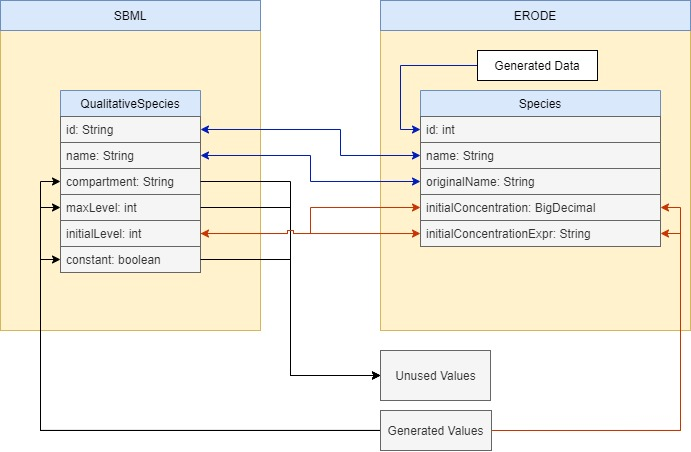
\includegraphics[scale=0.45]{Sections/Images/SpeciesConversionMapping.jpg}
    \caption{Species conversion mapping schema}
    \label{speciesConversion}
\end{figure}

When looking at figure \ref{speciesConversion}, it can also be seen that the species representation used by SBML, which can be found on the left side of the figure, has more attributes than the ERODE representation on the right. This is due to the fact, that ERODE specifies these values implicitly.
Firstly, ERODE does not support declaring species as \emph{constants}. This can only be handled implicitly, for example by not giving those species an update function that would make a value-change possible. Secondly, the \emph{maximum level} is already defined, since ERODE only is capable to represent models within the Boolean domain $\{0,1\}$. Making a successful conversion of a multi-valued network impossible in ERODE's current state. Finally, the \emph{compartment} attribute is a value simply cannot be translated to ERODE format. However, upon speaking with the ERODE's developers about this problem, it was decided that all models can be interpreted as single-compartment models, making this attribute irrelevant. Due to these reasons, these three SBML attributes can be safely discarded during the species conversion to ERODE format. Of course, this also means that these attributes require the generation of default values, when converting back to ERODE format. These default values are:
\begin{itemize}
    \item A default compartment name, that is the same for each species, such as "default"
    \item A maximum level of 1, due to all models being in the Boolean domain.
    \item The \emph{constant} attribute being set to \texttt{false}, as species without transitions cannot \\ change value, even if it is allowed.
\end{itemize}

Finally, the last attribute that needs special treatment during the conversion from SBML to ERODE is ERODE's \emph{id}-attribute. This value is used to give each species a unique identifier within ERODE itself and therefore has no counterpart in SBML. To provide such a value, the converter can simply start a counter during the species conversion, which is incremented each time another species has been converted. Since the counter value changes to a new value after each iteration, the counter value can be used as an \emph{id} for the ERODE species.



%As it can be seen in the conversion schema above, not all attributes of an SBML-species are required in ERODE, which means that they have to be discarded during conversion. Discarding data during conversions is always dangerous, as it can severely impact the quality of the conversion. Seeing that the SBML-attributes \emph{compartment}, \emph{maxLevel} and \emph{constant} are discarded, means that there are a few limitations to which kinds of networks can be converted to ERODE format correctly. \comg{The last sentence needs to be rewritten better. Break it into two sentences.}.\comg{Particularly, the limitations identified during our analysis are summarized in the following:}

%\begin{itemize}
%    \item All species in the network must be in the same compartment, therefore multi-compartment networks cannot be represented correctly. 
%    \item A maximum value of a species cannot be specified, which means that multi-valued networks cannot be represented in ERODE. 
%    
%    \item ERODE species cannot be constant. This means that the species update function (transition) needs to ensure that its value never changes, in order to represent the species correctly. 
    
%\end{itemize}
%Another problem that can arise, when converting an qualitative Species to ERODE format, is that ERODE requires an \emph{initialConcentration} \comg{In ERODE the initial value is also an optional attribute!}. In SBML this corresponds to the \emph{initialLevel}-attribute, which is an optional attribute. This means, that a default concentration needs to be generated by the converter, in case the \emph{initialLevel} is unset in SBML.

%When converting ERODE data to SBML format, it is also evident that ERODE cannot supply all data required by SBML. Luckily, this is not a problem, since most of the missing data are given by ERODE's restrictions to its supported models or are optional data in SBML. For required fields in SBML, that do not exist in ERODE, it is possible to assign default values, as they are defined by ERODE's limitations. The \texttt{constant}-field can be assigned the value \texttt{false}, since species in ERODE do not have a \textit{constant}-property. Also, all ERODE models are represented in a single compartment, which means that every species can be assigned to the same compartment, when converting to SBML. The last missing property, the maximum level is an optional parameter in SBML, but can be assigned a default value as well. Since ERODE currently only support BNs, the values of each species are restricted to the Boolean domain ${0,1}$, which means that the maximum level could be set to $1$ by default, but this is not required for a successful conversion. 

\subsection{Transition conversion}
Converting a transition from SBML to ERODE is much simpler than the conversion of a species, since ERODE requires a lot less data from the SBML representation. The drawback of this is that the converter needs to generate a lot more data, when converting back to SBML. This is due to SBML being an extensive format, that can be used to represent a large variety of model types.

as shown in figure \ref{fig:transitionConversion}, the conversion of an SBML transition to ERODE format requires a reference to the updated species and an update condition to be supplied. In SBML these attributes are contained in the \emph{outputs} and \emph{function terms} of a transition. The \emph{outputs} are a list containing references to each species updated by the given SBML transition. The \emph{function terms} are a list of items representing the condition, when to apply which result level. Since ERODE only supports models from the Boolean domain, only the function term for the result level $1$ (true) is required, since ERODE handles the \emph{otherwise}-case implicitly. 

Before a \emph{function term} can be used to represent a ERODE transition, the logical expression it contains must be converted to ERODE format. This is required, because both formats use different implementations to represent abstract syntax trees (ASTs), a data structure used to express mathematical expressions unambiguously.
Once the expression has been converted, the resulting expression (the update function) is used to create an entry in the LinkedHashMap, for each species referenced in the list of outputs. This creates a dictionary in ERODE, that can be used to look up, which species require which condition to be true, to change to the \emph{true}-state.

\begin{figure}[H]
    \centering
    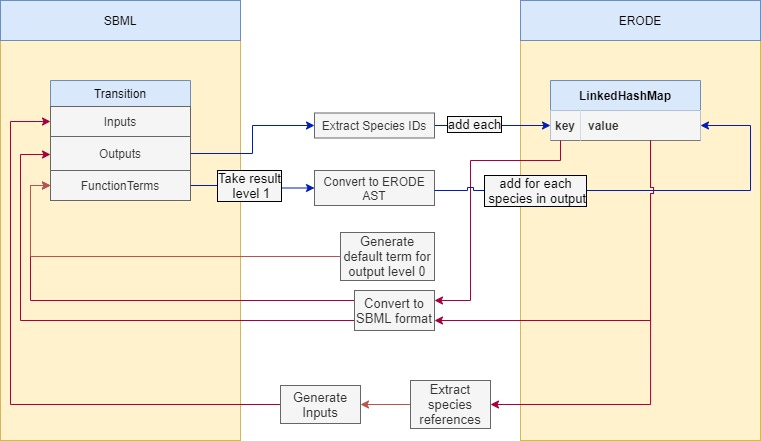
\includegraphics[scale=0.45]{Sections/Images/TransitionConversion.jpg}
    \caption{Converting transitions between SBML and ERODE}
    \label{fig:transitionConversion}
\end{figure}

When converting to SBML format, lists for the \emph{inputs}, \emph{outputs} and \emph{function terms} must be created for the generation of an SBML transition. The \emph{inputs} store information about the species referenced in the function terms of the transition. To generate an input-instance three pieces of information are required:
\begin{itemize}
    \item A string \emph{id}, to specify the unique identifier for the input
    \item The name of the variable used to reference a given species in the function term, stored in the \emph{qualitativeSpecies}-parameter
    \item A \emph{transitionEffect} that specifies how the input is affected by during the transition. This can always be set to \texttt{none}, since ERODE does not support transition effects.
\end{itemize}
To generate these \emph{inputs}, the converter needs to analyze the update function mapped to a species and find each variable used in the function expression. For each new variable found, a new input needs to be generated, duplicates can be skipped. This step is shown at the bottom of figure \ref{fig:transitionConversion}.

The list of \emph{outputs} stores similar information, but about the species that are modified by the transition. Just like \emph{inputs}, each \emph{output} requires an \emph{id}, a reference to a \emph{qualitativeSpecies} and the specification of a \emph{transitionEffect}. The only difference is, that the \emph{transitionEffect} needs to be set to \texttt{assignmentLevel}, since the values of the \emph{output}-species are overwritten by the transition. The only piece of information that is required from ERODE to generate an \emph{output}-instance, is the variable used for the species. The species references, which are used as keys in the \emph{LinkedHashMap}, can be used for the \emph{output}-generation.

Finally, to generate the list of function terms required by each transition instance, the update functions contained in the ERODE's hash map, can be used to genreate \emph{function terms} for the result level $1$ (true). This simply requires a format conversion of the AST represented in the update function. However, for the list of \emph{function terms} to be complete, another function term needs to provided. This is necessary, because SBML requires all possible outcomes of a transition to be defined by a function term. The converter must therefore generate a \emph{default term}, a special condtion-free function term, with a result level of $0$ (false). This \emph{default term} represents the \emph{otherwise}-case in the formal notation of a Boolean or multi-valued network.
Once all three lists have been generated, the converter can generate the converted SBML-transition.

Regarding the conversion between SBML and ERODE, all requirements for the conversion of Boolean networks have now been covered. For a deeper understanding of SBML (\cite{hucka2018systems}) and SBML-qual (\cite{sbmlqual2015}), it is therefore  recommended to take a look at their specifications.  and SBML-qual  specifications, which can be found at  \href{http://sbml.org/Documents/Specifications}{SBML.org} (\cite{documents/specifications}).

%Compared to the conversion of species, the conversion of transitions should be relatively easy, as both formats represent the same mathematical structure, a piece-wise logical function. The problem  is the fact that SBML is a format designed to support a much wider spectrum of network transitions than ERODE. This means, that there once again are limitations to, which SBML-transitions can be represented by ERODE accurately.
%The unsupported SBML properties in this case are, the \texttt{transitionEffect}'s for both transition \texttt{input}s and \texttt{output}s. Both transition effects define how the input or output are affected by the transition.

%In ERODE's network representations transitions do not affect transition \emph{input}s and assign their result to the transition \emph{output}. This is also supported by SBML by setting the transition effect of each input to \emph{none} and to \emph{assignmentLevel} for outputs. As the tranisition effect names might suggest, \emph{none} means that there is no effect on the inputs, whereas the \emph{assignmentLevel} transition effect will assign a new value to the output.
%Converting SBML-transitions can become problematic once the \emph{transition effects} differ from these mentioned cases. Instead of \emph{none}, input transition effects can be set to \emph{consumption}, which means that the \emph{input species} would be reduced during the transition, causing it to change value.  For outputs, the \emph{transition effect} could also be set to \emph{production}, causing the transition to add its result level to the output, instead of replacing it.
%Luckily, both the \emph{consumption} and the \emph{production} transition effects are typically be applied to \emph{multi-valued networks}, which are not supported by ERODE.
%\comg{The \emph{consumption} and \emph{production}, as input and output transition effects, refer to the Petri Net formalism wherein transitions consume tokes from input places.}
%If they were to be applied to a Boolean network in SBML, such a BN could not be represented by ERODE accurately, as the required operations to realize these transition effects are not supported.

%In order to actually convert a transition from SBML to ERODE format, given a correct conversion is possible, it simply requires the extraction of transition outputs and the function term with the result level of $1$ (true). Since all inputs already are referenced in the functions term and the input properties are reflected in it, the list of inputs is not required for the conversion of Boolean networks.
%Since each output references the species to be changed by its id, the only actual conversion step required, is the translation of the logical expression contained in the function term.

%This is a fairly simple operation, as the logical expression is given in the form of an abstract syntax tree (AST), that indicates the structure of the expression. In ERODE the same approach is utilized, just with different representations for the node in the AST. By translating each node in SBML's AST to a corresponding structure in ERODE, it is therefore possible to replicate the same AST in ERODE format, resulting in a converted logical expression.

%The final step is then to add the converted transition by adding it to the \emph{LinkedHashMap} storing all transitions (update functions) of the BN, by inserting the species ID, given by the transition output, as a key and adding the converted logical expression as the value mapped to the key.

%\begin{figure}[H]
%    \centering
%    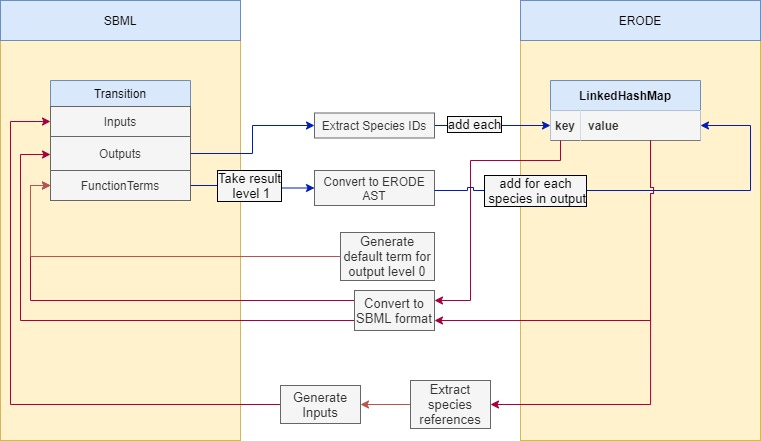
\includegraphics[scale=0.45]{Sections/Images/TransitionConversion.jpg}
%    \caption{Converting transitions between SBML and ERODE}
%    \label{fig:transitionConversion}
%\end{figure}

%As ERODE's transition format does not store any information about transition inputs outside of its function term, converting ERODE transitions back to SBML requires the generation of inputs, for the SBML transition.\comg{I think I can understand what you say here, but please be ore precise: for example. what is the ERODE's transition format.}
%This can be achieved by analysing the logical expression, collecting every new species reference it contains to species in the network. Once all inputs, outputs, and function terms have been generated from the ERODE data and stored in lists, it is then possible to generate the SBML transition from these lists.
%\comg{We can achieve the reverse conversion by following the steps:
%\begin{itemize}
%    \item We obtain from every logical expression (i.e. update function) the key (i.e. the output species).
%    \item We store them into lists.
%    \item Based on these lists, we generate the SBML transitions.
%\end{itemize}}

\subsection{Conversion of logical and relational operators}
Although the principle, how to convert a logical expression from SBML to ERODE format, is quite simple, the operator interfaces of both formats have not been taken into account so far. To be able to convert all valid logical expressions, it requires that all operators in one format, can be expressed using the available operators of the other format. To verify that this is indeed possible, an overview of both operator interfaces is required. The overview is shown in the following table:
\begin{table}[H]
    \centering
    \begin{tabular}{|c|c|c|}
    \hline
    Operator & SBML compatible & ERODE compatible    \\
    \hline
    AND $\land$ & \gcheck & \gcheck \\
    OR $\lor$ & \gcheck & \gcheck \\
    XOR $\oplus$ & \gcheck & \xcheck \\
    NOT $\neg$ & \gcheck & \gcheck \\
    IMPLIES $\rightarrow$ & \gcheck & \gcheck \\
    XNOR (binary equality) $\leftrightarrow$ & (\xcheck) & (\xcheck) \\
    EQUALS $=$ & \gcheck & \xcheck \\
    NOT EQUALS $\neq$ & \gcheck & \xcheck
    
\end{tabular}
    \caption{Operators usable in logical expressions for BNs and their support}
    \label{tab:operators}
\end{table}
When looking at table \ref{tab:operators} above, it can be seen the \texttt{XOR}, \texttt{XNOR}, \texttt{EQUALS} and \texttt{NOT EQUALS} operations are not supported by ERODE. This means that these missing operators need to be expressed using a combination of the existing operator set.

\subsection{The XNOR- and XOR-operation}
The \texttt{XNOR} operator does not exist in either formats, yet it could be used in logical expressions. SBML does not support the \texttt{XNOR} operator because it corresponds to a negated \texttt{XOR} ($\neg{\oplus}$) operation. Since both operators required to expression the \emph{XNOR}-operation already are supported by SBML, there is no need for a separate operator. ERODE, on the other hand, does not support the \texttt{XOR} operation. This means, it has to be constructed using the available operators.

Given two variables $P$ and $Q$, the \texttt{XOR}-operation is defined to be true, if either $P$ or $Q$ are true, but not both. In propositional logic, this condition can be expressed as: 
\[
(P \lor Q) \land \neg{(P \land Q)}
\]
\begin{table}[H]
    \centering
    \begin{tabular}{|c|c|c|c|c|}
    \hline   
    $P$ & $Q$ & $(P \oplus Q)$ & $(P \lor Q) \land \neg{(P \land Q)}$ & $P \oplus Q = (P \lor Q) \land \neg{(P \land Q)}$  \\
    \hline
    T & T & F & F & T \\
    T & F & T & T & T \\
    F & T & T & T & T \\
    F & F & F & F & T \\
    \end{tabular}
    \caption{Truth table verification that \texttt{XOR} is equivalent to $(P \lor Q) \land \neg{(P \land Q)}$}
    \label{tab:verified_xor}
\end{table}
As it can be seen in the truth table \ref{tab:verified_xor} above, the two logical expressions are equivalent, which means that the \texttt{XOR}-operation can be translated to ERODE format using its supported operators.

\subsection{Equality and inequality operators}

Just like the \texttt{XNOR}-operation, the inequality operation can be constructed by negating the equality operator. However, neither equality operator is currently supported by ERODE. Fortunately, the equality can be expressed differently, depending on the domain it is used in.

In the Boolean domain, the \texttt{XNOR}-operation also represents binary equality: it is true if both sides are true, or both sides are false. Since \texttt{XOR} is the opposite of \texttt{XNOR}, the \texttt{XOR}-operator must be equivalent to the inequality-operator. So the big question is, why not just translate these operators to their corresponding logical equivalents?

To answer this question, it is necessary to take ERODE's current state into account. The program is under development and it is intended to implement support for multi-valued networks. In other words, ERODE will eventually support models outside the Boolean domain. Since this converter should be able to convert SBML-qual models into ERODE format, it would be wise to design the converter such that the changes required to adapt to new version of ERODE are minimal.

Since ERODE is restricted to the Boolean domain and these relational operators need to be supported; A good midway would be to implement them in the Boolean domain, while making them as independent from the other operators as possible. This means finding an expression, that has a minimal overlap with the \texttt{XOR}- and \texttt{XNOR}-operators.

This can be realized using the \texttt{implies}-operator. This is due to the fact, that logical equality also corresponds to the \emph{if and only if}-conditional ($\leftrightarrow$) in propositional logic. The conditional can be expressed using the \texttt{implies}-operator, thereby making it highly independent from the other operators.
\[
    A \leftrightarrow B = (A \rightarrow B) \land (B \rightarrow A)
\]
To prove that $(A \rightarrow B) \land (B \rightarrow A)$ only is true, when $A$ and $B$ are equal, consider the possible outcomes of an implication:
\begin{table}[H]
    \centering
    \begin{tabular}{|c|c|c|}
        \hline
         A & B & $A \rightarrow B$  \\
         \hline
         T & T & T \\
         T & F & F \\
         F & T & T \\
         F & F & T \\
         \hline
    \end{tabular}
    \caption{Outcomes of an implication given $A$ and $B$}
    \label{tab:implies}
\end{table}
As it can be seen in table \ref{tab:implies}, the only way for an implication to be false, is when the first argument is true and the latter false. This is also, why $(A \rightarrow B) \land (B \rightarrow A)$ cannot be true, when the two arguments are different, as shown below.
\begin{align}
    &A \rightarrow B &= F \\
    &B \rightarrow A &= T \\
    \hline
    &(A \rightarrow B) \land (B \rightarrow A) &= T \land F & &\text{from (4.1) and (4.2)} \\
    &T \land F &= F& &\text{from (4.3)}\\
    \hline
    &(A \rightarrow B) \land (B \rightarrow A) &= F& &\text{from (4.4)}
\end{align}

Since it has been shown, that equality can be expressed as $(A \rightarrow B) \land (B \rightarrow A)$ in the Boolean domain, it is also evident that inequality would be its negation, This means, that the required relational operators can be converted from SBML to ERODE without having great similarity to the \texttt{XOR}- and \texttt{XNOR}-operators.

It has now been shown that all supported by SBML can be expressed using a combination of ERODE's operators. Unfortunately, these expression conversions cause a significant loss in readability, due to their lengthiness. The expression length problem is especially severe, when it comes to the \emph{equality} and \emph{inequality} operations, since these are used very frequently in the SBML format. Their high usage is due to the fact that many networks are represented using a multi-valued notation (integer based notation) restricting the model to use comparison operations, for operations on variables and constants. This also extends to networks that are within the Boolean domain, as all Boolean models are a subset of all the possible multi-valued models.

To solve the problem of lengthy and unreadable expressions, it would require to update ERODE and extend its operator interface. With this update, the original expression could be maintained and the conversion would have no impact on its readability. Once the developers were presented with this problem, they did eventually decide to extend the operator interface to support the same operator set as SBML. 
\clearpage 
\chapter{Design}
%Overall design goals:
%The converter is open to extension and modification
%The code should be easy to extend and modify
% - Requires code that is easy to understand
Now that both data formats have been analyzed and conversion schemes have been proposed, a system can be designed to support this conversion. This section will explain the system architecture and its design process. Initially in section 5.1, a framework system is designed that deals with the practical requirements and limitations of the conversion and acts as a container for the conversion modules. Such requirements and limitations include considering how to exchange data with the converter. Section 5.2 gives an overview of the design goals that are rooted in aesthetics and propose design approaches how to achieve them. Such design goal include ease-of-use (simplicity) and maintainability (code management). Section 5.3 presents how the system's component structure divides the conversion process into multiple steps. Section 5.4 shows how a certain independence between those components can be achieved. Finally, the base structure of the converter components is explained in section 5.5.


%\comg{We now proceed to the design of the system to support the conversion between the two data formats.} This section will explain the system architecture and its design process, starting by showing how the base system is rooted in its requirements. Then, the level of detail will increase step by step, by looking at the design of various converter components. This way, the underlying design ideas will be revealed before diving into the details of the system.

%\commentGeorgios{This section includes a high level of technicality and it is difficult for the reader to understand. Be more specific and explain in a great level of detail what is the goal of each subsection. For example: In 5.1, we recast the requirements of the system to be build after considering our initial proposal and the research conducted in the analysis section. In subsection 5.2, we specify the development goals and base our design approach to some good software engineering practices. Section 5.3 does this with 1-2 sentences. Section 5.4 does this with 1-2 sentences. Section 5.5 does this. Moreover, about 5.3,5.4,5.5 take care of the order of presenting these sections. I understood more or less what you did, but your goal is to help, guide, and facilitate the reader to understand what you did..}

\section{System requirements and limitations}
The most basic requirement of the converter, is that it must be able to convert SBML-qual to ERODE-format and vice versa. To do so, the converter must be capable of basic input/output of files (file-I/O), as a standalone program. Once the converter has read its input file, it must be able to extract the required data from the file. For SBML this can be done using the JSBML-library, a Java-API to read and write SBML files. In case of the ERODE format, the ERODE-library is capable of file-I/O, but only to the extent of writing. This means, that the standalone converter can only generate ERODE-files from an SBML input, but not vice versa. The compiler used to interpret the ERODE format (.ode) is also not publicly available, which is why there are no means to parse ERODE-files directly in the converter.
However, the converter must still be able to converter ERODE's data representation into SBML format, since it still could be used inside ERODE to export to SBML. To enable the converter to convert from ERODE to SBML, the reading and writing of files, simply needs to be separated from the conversion process itself. In other words, by converting between the data representations used by ERODE and JSBML. This will essentially outsource all file-I/O to the JSBML and ERODE plugins, and turn the converter into a bridge between the two formats. 

\begin{figure}[H]
    \centering
    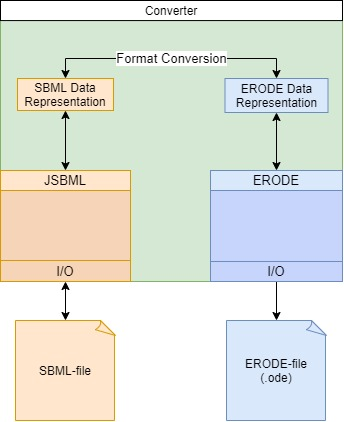
\includegraphics[scale=0.45]{Sections/Images/ConverterSystem.jpg}
    \caption{An overview of the conversion system}
    \label{fig:converter_overview}
\end{figure}

As shown in figure \ref{fig:converter_overview}, the converter will be given an SBML file to convert. The converter will then take the data representation of the file and convert it to the other data representation, which then is written to a file. When integrated into ERODE, the converter will be given directly from the host program, and generate an SBML file representing the given model as output.

\section{Development goals and design approach}
Now that the basic system has been designed based on its requirements, it is time to think about how such a system can be realized in practice. That means deciding:
\begin{itemize}
    \item How file-I/O should work in this system.
    \item How the data conversion component should be designed and structured.
    \item How modifiable the system should be.
\end{itemize}
For the standalone converter, the first question is relatively simple to answer. Since both the JSBML- and the ERODE-plugin are contained within the converter, the converter itself must have a file-I/O interface of its own. This interface must be able to take in an SBML-file as an input and return a new ERODE-file as output.

The answers to the second and third question are intertwined, as the design of the conversion component will define how dependent the converter will be on the current state of both formats. Since the ERODE-tool still is in development and therefore subject to change, the converter should have a design that easily can be adapted to support changes in both formats. This requires the converter to be designed in a way that is both easy to maintain, whilst being highly modifiable.

This can be achieved using the SOLID-principle, which consists of the basic rules to create highly maintainable and extendable applications using object oriented programming. The principle itself is a collection of five principles:
\begin{itemize}
    \item \textbf{S}: The \textit{single responsibility principle} states that software components should be kept small and dedicated towards a single specific task. This will keep code segments shorter, as well as easier to understand and change.
    \item \textbf{O}: The \textit{open-closed principle} states that existing software components should be open to extension but closed for modification. This means, that any existing functionality of a component should remain unchanged, as any changes may impact the whole system. In this the case of the converter, it may not always be possible to ensure that the design always follows this principle. Since the conversion formats still are being developed, it may become necessary modify existing functionality of the converter to adapt to changes in both formats.
    \item \textbf{L}: The \textit{Liskov substitution principle} states that components that are derived from other components should be able to replace the component they were derived from without causing unexpected results.
    \item \textbf{I}: The \textit{interface segregation principle} state that interfaces should never force components to support interface-methods that should not be supported by the component. Instead such an interface should be broken down into smaller ones that can be implemented selectively.
    \item \textbf{D}: The \textit{dependency inversion principle} states that components should depend on interfaces instead of direct dependencies. This increases their independence and allows components that implement the same interface to be used interchangeably.
\end{itemize}

It should be remarked that these definitions are based on the SOLID definitions given in \href{https://learning.oreilly.com/library/view/apex-design-patterns/9781782173656/ch01s10.html#ch01lvl2sec8}{Apex Design Patterns} by \emph{Jitendra Zaa} and \emph{Anshul Verma}

\section{Converter layering}
The analysis of SBML-qual in section 4.2 revealed the complex multilayered structure of the SBML-format. Due to the complexity, the conversion to and from SBML is therefore quite an extensive task. However, this task can be broken down in to smaller sub-tasks by separating the layers and converting them in different converter components. This layer separation also reduces the responsibilities of each converter component, since each component only operates on a single layer. This enforces the \emph{single responsibility principle}.

%During the analysis of SBML-qual it quickly became visible that SBML-qual models are fairly complex structures consisting of many layers. By creating a separate converter component for each of these layers, the conversion process can be broken down into multiple smaller steps. This makes each component responsible for a single layer of the SBML-qual structure in the conversion process, enforcing the \emph{single responsibility principle}.

%\comg{A preliminary analysis of SBML-qual revealed the multilayered complex structure of the SBML-format. We initially broke down the conversion process into multiple steps. Each step consists of a separated component converter dedicated to each layer. In other words, each component is responsible for a single layer of the SBML-qual structure in the conversion process satisfying the \emph{single responsibility principle}.}
\begin{figure}[H]
    \centering
    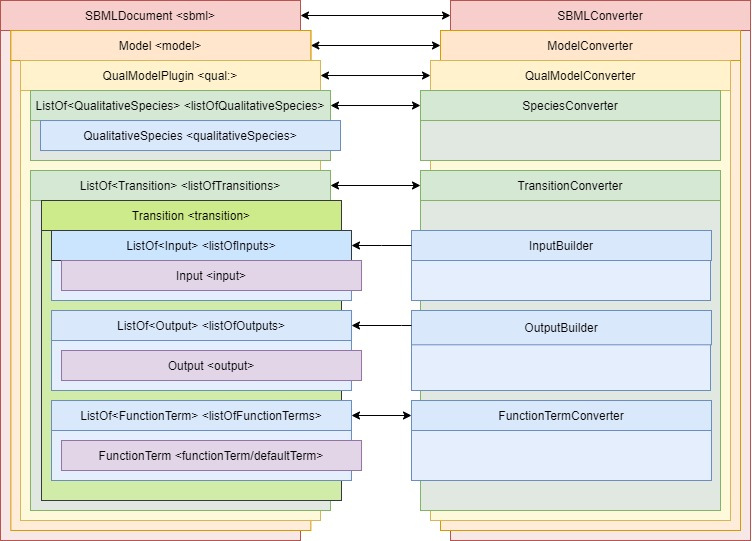
\includegraphics[scale=0.45]{Sections/Images/ConverterLayering.jpg}
    \caption{Mapping of SBML-qual layer to corresponding converter component}
    \label{fig:converterLayering}
\end{figure}
Figure \ref{fig:converterLayering} shows the SBML-qual structure to the left and the converter's component structure to the right. Components that are enclosed by an outer component, are contained within their outer component. The coloring indicates which components are located within the same layer. The arrows are used to indicate which of the converter's components are responsible for the conversion of specific layer in the SBML-qual structure. As an example, the \emph{ModelConverter} is responsible for the conversion of the \emph{Model}-layer in SBML-qual.

The arrows also indicate, which conversion the various converter components are responsible for. Arrows pointing at the converter indicate that the component is responsible for the conversion of SBML to ERODE format. Arrows pointing at the SBML-qual structure indicate the opposite, the conversion from ERODE to SBML-qual.

Components in the SBML-qual structure that are not connected to a converter component via an arrow, are converted as a part of their enclosing layer. This also counts for SBML-layers that only are pointed at by a converter component. For example, each \emph{input} (<input>) is converted as a part of the list of inputs (<listOfInputs>) it is contained by. The list of inputs is generated by the \emph{InputBuilder}, when converting to SBML-format, but it is converted as a part of each transition, when converting to ERODE's format.

The reason, why some of these layers are converted along with their outer layers is that the outer layer for one or both conversion directions, simply does not contain enough data of its own. For example, list are used to contain multiple item of the same type, but apart from these items they contain no relevant data of their own.

%Figure \ref{fig:converterLayering} shows the layer separation achieved by mimicking the SBML-qual structure using the converter components.\comg{explain the figure better. The left part of the figure displays this. the right part of the figure displays this. The arrows indicate that...} The arrows indicate, which component is responsible for which SBML-qual layer and \comg{the nature of the responsibility} what kind of responsibility it is. \comg{ERODE does not require data from each layer of the SBML-structure, so the converter allows unnecessary layers to be omitted in the conversion process. Hence, we use two-way connections to } Two-way connections indicate that the responsible converter component is responsible for both conversion directions (SBML to ERODE and vice versa), whereas the arrows pointing at the SBML-structure indicate that these components only are required during the conversion from ERODE to SBML. Instance layers, such as the \texttt{QualitativeSpecies}- or \texttt{Input}-layer are converted along with their enclosing list layer, as they only have the logistical purpose of containing multiple items of the same type.

Now that the overall converter structure has been designed, it is important to consider how the converter components interact with each other during the conversion. This requires a step by step analysis of the conversion process.
\begin{figure}[H]
    \centering
    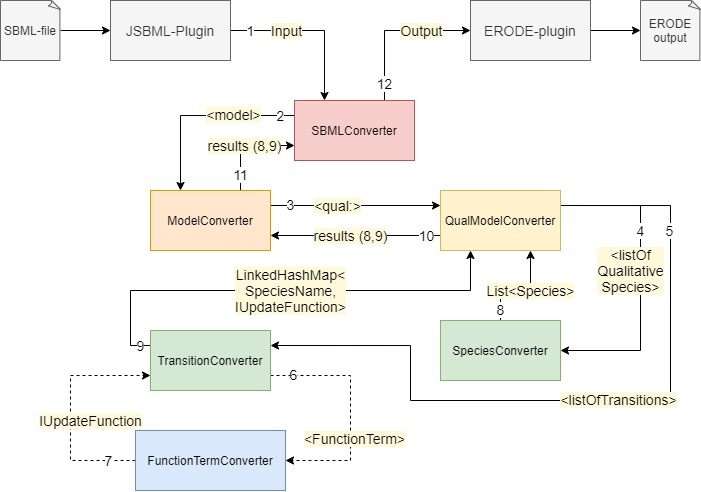
\includegraphics[scale=0.45]{Sections/Images/SBMLConversion.jpg}
    \caption{SBML to ERODE conversion process}
    \label{fig:SBMLConversion}
\end{figure}
As shown in the steps 1-3 of figure \ref{fig:SBMLConversion}, the outer converter components simply remove the outer-most layer of the SBML-qual input they are given and pass on the remaining data to the next component. This is the only requirement for the first two components since the outer SBML-layers contain only meta-data about the model, which is not required by ERODE. Thereafter, the \texttt{QualModelConverter} splits the data representation as shown in steps 4 and 5, since species and transitions are independent structures that do not require data about the other during their conversion. Because species do not contain sub-layers, the \texttt{SpeciesConverter} can convert each species and return a list of all species in ERODE format to the \emph{QualModel converter} (steps 4 and 8).

To convert transition and additional conversion step, the conversion of \emph{function terms}, is required. This is handled by the \emph{FunctionTermConverter} in steps 6 and 7, which receives a \emph{function term} from the \emph{TransitionConverter} and returns the function expression within as an \emph{IUpdateFunction}. The \emph{IUpdateFunction} is the corresponding structure in ERODE. The steps 6 and 7 are highlighted using dotted arrows, as they have to be repeated for each single transition. This means that these steps will run on a loop until all transitions have been converted.
In steps 8 and 9, the species and transitions are then returned in ERODE format, which then are routed back to the conversion entry/exit point in the \texttt{SBMLConverter}. As a final step, the \texttt{SBMLConverter} will then package the converted ERODE structures into an ERODE model, which is passed on to the ERODE plugin to generate the file.

Apart from a few minor details, the reverse conversion, from ERODE to SBML, largely corresponds to the execution process in figure \ref{fig:SBMLConversion}, but in reverse. The main differences are the the \emph{input} and \emph{output} builders from figure \ref{fig:converterLayering} need to be included to generate SBML transitions and that the ERODE model is supplied by the ERODE host program instead of a file.

\section{Component separation}
When looking back at, how each of these converter components exchange data, it quickly becomes visible that all components request data from components in a lower layer (sub-components), whereas they always respond to a component in a higher layer (parent). Since that is the case, all components can be separated by introducing interfaces that define the contract for their communication. This enforces the \emph{dependency inversion principle} and increases the maintainability of the converter even further, by design.
\begin{figure}[H]
    \centering
    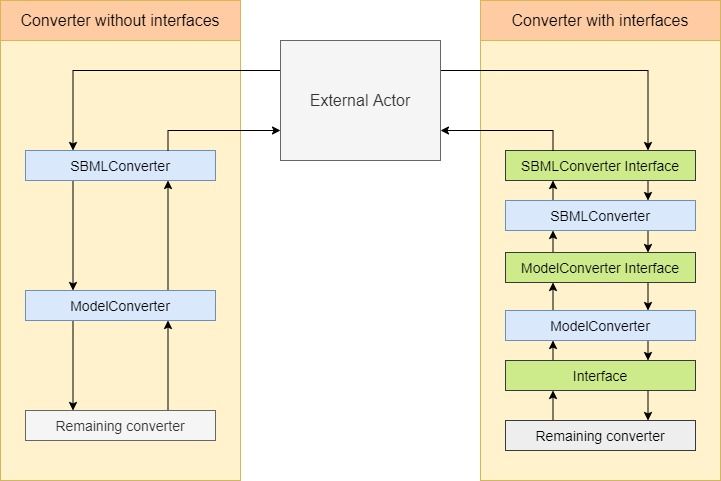
\includegraphics[scale=0.45]{Sections/Images/Interfacing.jpg}
    \caption{Converter structure with and without interface}
    \label{fig:interfacing}
\end{figure}
When comparing the two converters shown in figure \ref{fig:interfacing} it can be seen that the converter without interfaces consists of components that depend on each other directly, this means that there is one specific type of component that is required to ensure the conversion can succeed. 
The other converter on the other hand relies on interfaces, which act as contracts of interaction. Since it relies on interfaces instead of a direct dependency, components are implemented completely independent of each other. Implementations are hidden by the interface allowing components that implement the same interface to be used interchangeably.

\section{Component structure}
Another way of increasing maintainability by design, is to divide each converter component into sub-components. Since each component currently is responsible for both conversion directions, they can be divided into separate pieces internally. From the outside there still is only one component to interact with, but internally the two ways of conversion are handled by different sub-components.
To facilitate this, each component would require some kind of manager that can identify, which conversion process is required and initializes it accordingly.
\begin{figure}[H]
    \centering
    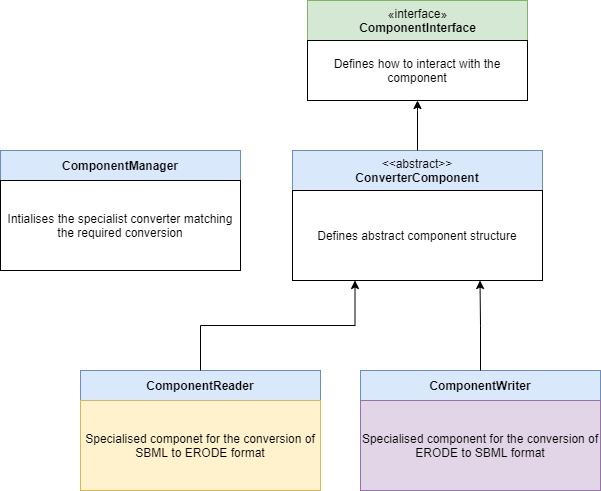
\includegraphics[scale=0.45]{Sections/Images/ComponentStructure.jpg}
    \caption{General component structure}
    \label{fig:component}
\end{figure}
As it can be seen in figure \ref{fig:component}, each component is controlled by a manager that initializes the required conversion unit. The possible interactions with the conversion unit from outside the component is defined by the \emph{ComponentInterface}. The interface is implemented by the \emph{ConverterComponent}, an abstract class defining the general converter unit's object-structure. The \emph{ConverterComponent} is extended by the \emph{reader}- and \emph{writer}-units, which define the specialized conversions of both formats. 

All conversion unit \emph{readers}, take care of \emph{reading SBML}, converting it to ERODE format, whereas \emph{writers} take ERODE format as input, \emph{writing} it to SBML. This naming convention is used to indicate the conversion direction for each of these components without needing to use either SBML or ERODE as a part of the class' name.
It should be added that this general structure may vary slightly from component to component, as some components may require additional functionality, which according to the SOLID-principle would need to be added as separate entities.
%As shown in figure \ref{fig:SBMLConversion} each converter will consume the outer most SBML-layer and pass its sub-components on to the next converter. The SBML-layer passed on is indicated by the highlighted SBML-tag on each link in the figure, e.g the \texttt{<model>} on link $2$. The converters at the lowest level will the convert their SBML-data to ERODE format first, pass the converted data back to their parent-converter. Keep in mind, that steps $6$ and $7$ might occur multiple times on a loop, as most Boolean networks consist of multiple transitions. Once, the low-level conversion is completed, the parent converters will then pack the returned ERODE-data into the required ERODE-structures. Since the packing of ERODE structures requires less layers than SBML, the remaining top-level converters will simply route the data out of the conversion module, so that it can be printed to the output-file by the ERODE-plugin. These routing steps are indicated by the \texttt{results} links.
%When considering the various steps of the conversion process, it is clear that the system in its current form is well suited to convert SBML-qual to ERODE format. On the other hand, when it comes to the reverse case, where the ERODE-format is converted to SBML-qual, the system design becomes flawed. In its current state (see figure \ref{fig:converterLayering}) the \texttt{TransitionConverter} converts the list of transitions and is also responsible for the conversion of inputs and outputs in each of these transitions. For a conversion from SBML-qual to ERODE, this is a fine amount of responsibility as most of the input and output data simply is discarded. However, for the reverse conversion these structures need to be generated by the converter, which is a big task, giving the \texttt{TransitionConverter} too much responsibility.
%Although the primary purpose of this project is to create a converter between the formats SBML-qual and ERODE, there are a few details that should be kept in mind during the design and implementation of the converter:
%\begin{itemize}
%    \item At the point of writing, ERODE only supports BNs, which requires the converter to be highly modifiable.
%    \item Since both the converter and ERODE are implemented in Java, the converter should be easy to integrate.  
%\end{itemize}
%\subsection{Design approach}
%Even though there are many ways to design a highly modifiable converter that is easy to integrate. Simplicity, is what needs to be at the core of the solution. This can be achieved by following principles like the \emph{Single Responsibility Principle}, the \emph{Principle of Least Knowledge (Law of Demeter)} and following best practices, when it comes to writing clean code, such as those presented in the book "Clean Code - A Handbook of Agile Software Craftsmanship" by Robert C. Martin.
%Add references to sources
%\subsection{Tree conversion}
%The SBML is structured as a tree with many branches
%Since ERODE only works with SBML-qual, only a small subtree of the SBML structure is relevant for conversion
%In order to convert back to SBML from ERODE these structures must be created

%The converter must be able to do 3 things
% - Extract and unpack SBML/ERODE data
% - Convert data into the format of the other
% - Pack and export data (adding header information if required)

%To keep the conversion simple:
% Follow the Principle of least knowledge (Law of Demeter) and the S of SOLID principles
% Single Responsibility principle
%   - "a class should have only one reason to change"
%   - One class one responsibility/purpose

%Principle of least knowledge
%   - A class should only know what is absolutely needs to know
%   - Independent data should be handled by independent classes

%By attaching a converter class to each node in the SBML-tree, the highest possible data independence will be achieved

%\begin{figure}
%    \centering
%    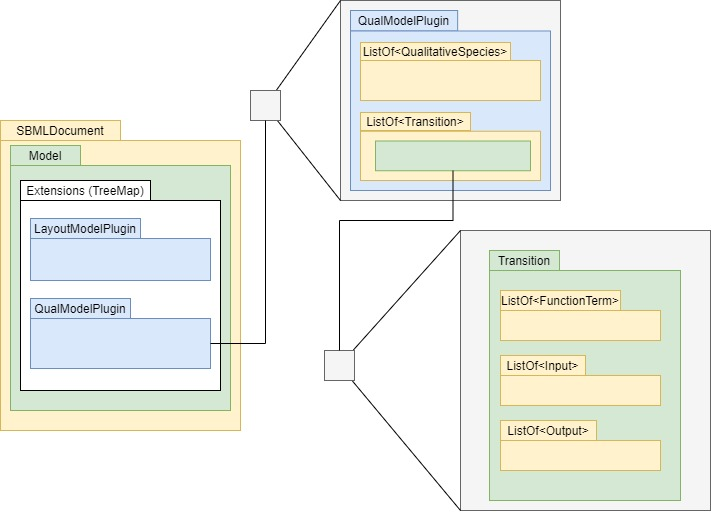
\includegraphics[scale=0.4]{Sections/Images/SBMLModel structure.jpg}
%    \caption{The SBML model reduced to its most important components}
%    \label{fig:my_label}
%\end{figure}

%Side Notes:
%Law of Demeter - Principle of least knowledge
\clearpage 
\chapter{Implementation}
Now that the analysis of the conversion and the converter design is complete, it is time to consider the converter's implementation. A substantial part of the converter system can be implemented by simply creating a java structure corresponding to the conceptual structure given in the design section. For example, a converter component could be realized as a package containing classes and interfaces, which define its sub-components. The tasks performed by each of these components could then be implemented as methods in the corresponding classes, according to the conversion rules specified in the analysis. However, when it comes to implementations there are often multiple ways to achieve the same goals and sometimes practical limitations that can prevent you from using a certain approach. 

In this section, some of the most prominent implementation choices will be showcased to give an understanding how the converter was realised and how some practical challenges have been solved. Section 6.1 will explain, how the component design given in section 5.5 is implemented by showcasing the \emph{ModelConverter} component. In section 6.2 it will then be explained how to convert function terms between the two formats.

\section{Component construction}
From the component design shown in figure \ref{fig:component}, it can be seen that the \emph{manager} and the \emph{interface} are the only independent structures of a component, since all other components inherit from the interface. These two structures are also the only ones, that are visible to the outside. 

The reason for this is, that the other structures contain information about the components implementation, which according to the SOLID-principles should remain hidden to the outside.
As such, the \emph{manager} also needs to act as an entry point for outside data, since this data is required for the converter initialisation. Due to the component's structure, it is also the only possible way to handle this, since the \emph{interface} cannot be accessed before the converter itself has been initialised. This only leaves the \emph{manager} as an entity that is accessible from the outside.

\subsection{Showcase ModelConverter}
When looking at the contents of the \emph{model}-package of the converter, it can be seen that it consists of the five entities specified in the component design.
\begin{figure}[H]
    \centering
    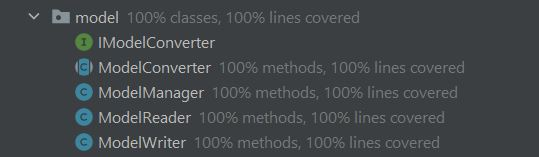
\includegraphics{Sections/Images/ModelConverter.JPG}
    \caption{The contents of the model-package}
    \label{fig:modelConverter}
\end{figure}
The \emph{IModelConverter} is the interface that specifies the methods that can be used to interact with the component.
\begin{figure}[H]
    \centering
    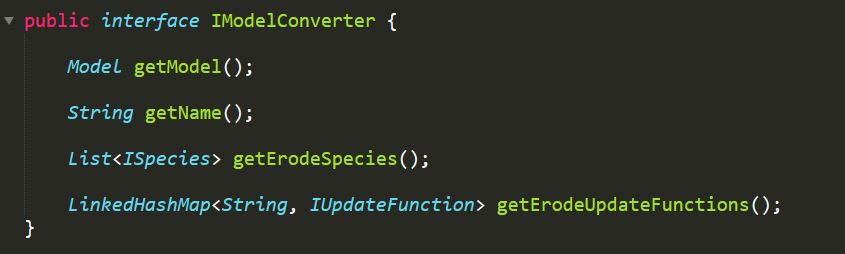
\includegraphics[scale=0.8]{Sections/Images/ModelInterface.JPG}
    \caption{The \emph{IModelConverter}-interface}
    \label{fig:modelInterface}
\end{figure}

As it can be seen in figure \ref{fig:modelInterface}, the interface consists of four methods that can retrieve data from the component. The \texttt{getModel()}-method returns a \texttt{Model}-object, which is the SBML-structure containing the data of an SBML-model. The \texttt{getName()}-method is used to retrieve the name of the model from the given network. Since the representations of both formats store the name of the network, it was added as a separate method, to allow format independent access to that value. The last two methods in the interface, the \texttt{getErodeSpecies} and the \texttt{getErodeUpdateFunctions}, are used to retrieve the data structures for species and transitions (update functions) in ERODE format.

This interface is then implemented by the abstract class \emph{ModelConverter} shown in figure \ref{fig:abstractModel}, which specifies the set of fields both converter units have in common and it provides constructors to initialise them. Since it is an abstract class, it cannot be initialised itself, but the constructors can still be utilized by its derived classes.
\begin{figure}[H]
    \centering
    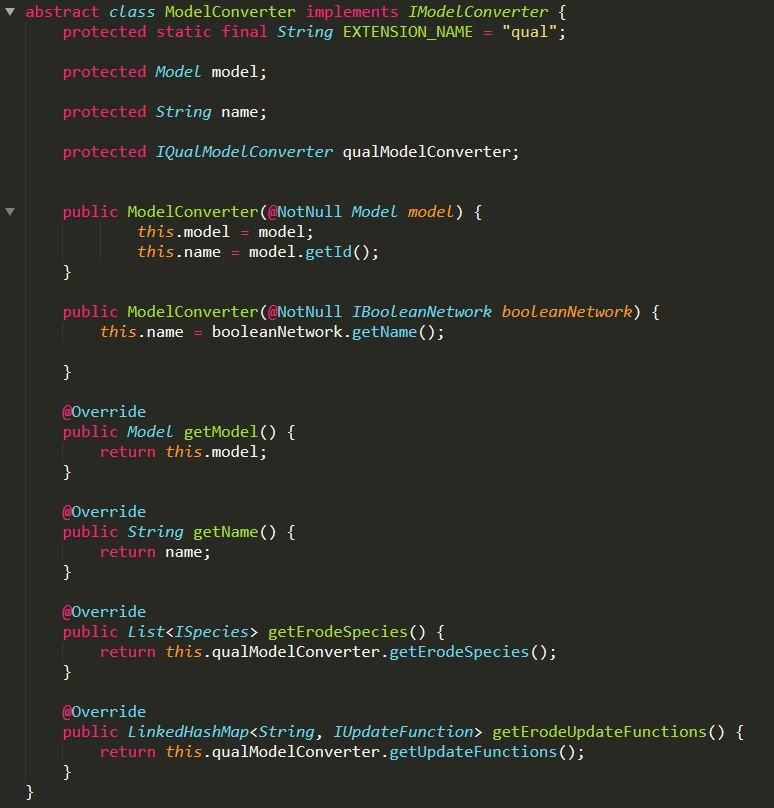
\includegraphics[scale=0.8]{Sections/Images/AbstractModel.JPG}
    \caption{An overview of the abstract \emph{ModelConverter}-class}
    \label{fig:abstractModel}
\end{figure}
The \emph{ModelConverter} enforces the \emph{dependency inversion principle} as the only converter reference is via the \emph{IQualModelConverter}-interface. Since nothing but the interface is known to the \emph{ModelConverter}, the internal logic of the \emph{QualModelConverter} remains hidden.

The \emph{ModelConverter} base class is extended by the \emph{ModelReader} and the \emph{ModelWriter}, which define the two ways of conversion. Both classes contain a constructor and a set of private methods designed to deal with the specifics of their conversion.

\begin{figure}[H]
    \centering
    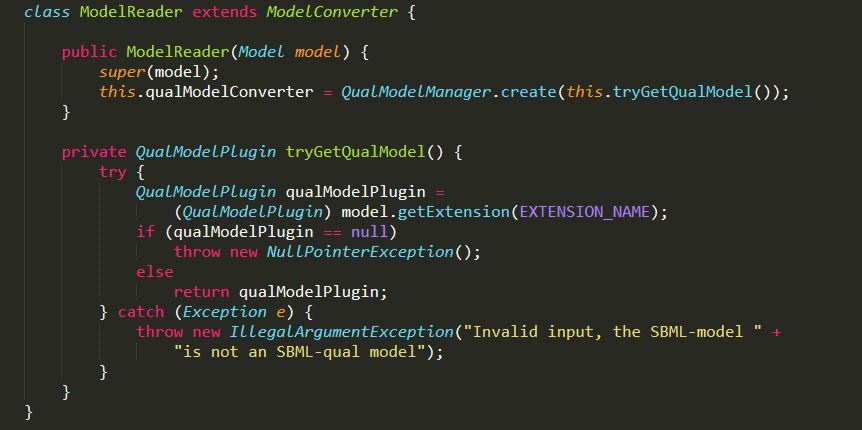
\includegraphics[scale=0.75]{Sections/Images/ModelReader.JPG}
    \caption{The \emph{ModelReader-class}}
    \label{fig:modelReader}
\end{figure}

\begin{figure}[H]
    \centering
    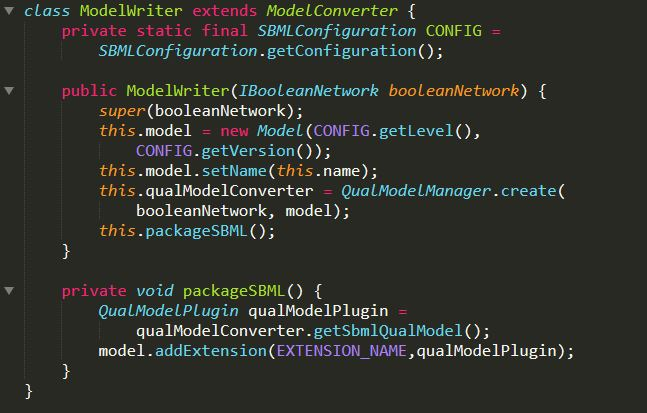
\includegraphics[scale=0.75]{Sections/Images/ModelWriter.JPG}
    \caption{The \emph{ModelWriter}-class}
    \label{fig:modelWriter}
\end{figure}

When looking at the figures \ref{fig:abstractModel} through \ref{fig:modelWriter}, one might notice that none of these classes have the \emph{public} modifier. This enforces that their visibility is limited to the package they are contained in. Since each component is implemented in a different package, all non-public classes are therefore completely invisible to classes in other packages.

Lastly, the \emph{ModelManager} acts as an entry point for the converter. It implements two \texttt{create()}-methods, which take care of initialising the two different converters. Since each \texttt{create()}-method, takes an input, the input is used to define the type of converter to be returned.
As shown in figure \ref{fig:modelManager}, the first \texttt{create()}-method takes a \texttt{Model}-object as input, which is an object-type used by JSBML to represent SBML-models. Since this method is dealing with SBML-input, the converter capable of converting to ERODE is required. The second \texttt{create()}-method handles the reverse case, where ERODE-input is given and a converter that can convert to SBML is initialised.

\begin{figure}[H]
    \centering
    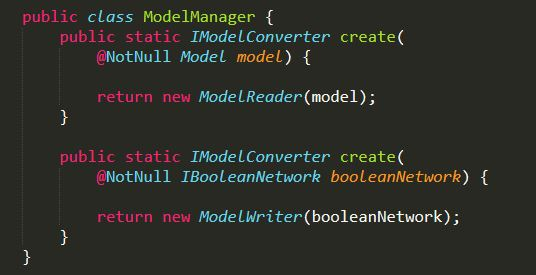
\includegraphics{Sections/Images/ModelManager.JPG}
    \caption{The \emph{ModelManager}-class}
    \label{fig:modelManager}
\end{figure}

\section{Function term conversion}
As shown in the analysis, the function term structure in SBML-qual defines the condition for a given transition result.
As such, it contains the \emph{result level} and the \emph{logical expression} forming the condition.
The logical expression is given in the form of an abstract syntax tree (AST), a structure used to represent the operation precedence in machines to avoid ambiguity.

Since both formats represent the transition conditions using ASTs, the primary task is to replicate the exact same tree-structure in the other format. The challenging part of this conversion is that different expressions have different AST-structures representing them. This means, that the converter must be able to analyze each element in the AST and select the correct conversion method for that element to ensure a correct conversion.
To solve this task, an algorithm is required that can traverse the AST, analyze each element and select the correct conversion method for it. Additionally a converter structure is required to execute the conversion of these elements.

In order to convert a given AST to another format, the conversion algorithm must be able to recognize the different elements that can occur in it. In general, every AST can be interpreted as a graph consisting of vertices (nodes) and edges (links). The vertices represent operators, variables and constants, whereas the edges indicate how these nodes are connected. Based on the amount of outgoing connections of a node, it is possible to divide nodes into three groups:
\begin{itemize}
    \item \emph{Binary} nodes representing binary operations with two outgoing connections
    \begin{figure}[H]
        \centering
        \begin{tikzpicture}[level/.style={sibling distance=60mm/#1}]
            \node [circle,draw,fill=red] (z){$\land$}
                child {node [circle,draw] (a) {$P$}}
                child {node [circle,draw] (b) {$Q$}};
        \end{tikzpicture}
        \caption{Binary node (red) binding variables}
        \label{fig:binaryNode}
    \end{figure}
    \item \emph{Unary} nodes representing unary operations that only have a single outgoing connection
    \begin{figure}[H]
        \centering
        \begin{tikzpicture}[level/.style={sibling distance=60mm/#1}]
            \node [circle,draw,fill=blue] (z){$\neg$}
                child {node [circle,draw] (b) {$T$}};
        \end{tikzpicture}
        \caption{Unary node (blue) with a single constant child node}
        \label{fig:unaryNode}
    \end{figure}
    \item \emph{Leaf}-nodes representing a variable or a constant, which have no outgoing connections
    \begin{figure}[H]
        \centering
        \begin{tikzpicture}[level/.style={sibling distance=60mm/#1}]
            \node [circle,draw] (z){$=$}
                child {node [circle,draw] (a) {$\neg$}
                    child {node [circle, draw, fill=green] (c) {$P$}}
                    }
                child {node [circle,draw, fill=green] (b) {$Q$}};
        \end{tikzpicture}
        \caption{Leaves (green) in an AST}
        \label{fig:leaves}
    \end{figure}
\end{itemize}

The components required to provide the conversion functionality can be structured in a similar fashion as the other converter components using the SOLID-principle. An abstract \emph{node converter} is introduced hiding the three different converter types to convert the three node types, which then again are split in two, to separate the conversion directions.

With the conversion infrastructure in place, it is now time to look for an algorithm that can handle the tree traversal during the conversion. In the case of ASTs, there are two approaches of traversal: The \emph{bottom-up} approach, where the tree analysis begins at the leaves, working its way up towards the root, and the \emph{top-down} approach, starting at the root, ending at the leaves.

From a performance point of view, algorithms using the bottom-up approach are have a better performance as they only need to traverse each node once. In top-down approaches the algorithms need to back-trace their steps to a previous node, as branches in the tree may split, forcing them to prioritise one node over the other.

In order to obtain the performance benefit fro the bottom-up approach it is required that the leaves of the tree can be accessed directly, and that children (lower-level nodes) have a reference to their parent (higher-level nodes). Both in SBML-qual and ERODE, the only directly accessible node is the root of the AST. This causes any bottom-up algorithm to lose its performance benefit, as they new require a data structure transformation to make the leaves of the AST accessible.

Due to the fact, that there is no performance loss and no additional structural transformation required, it is both viable and also much simpler to use a top-down approach. A suitable algorithm for such a tree traversal is a \emph{DFS} (depth-first-search). The algorithm will traverse down the branches of the tree, analyzing each node in the search for leaves. Since leaves have no children and can be converted instantly. In case a node is not a leaf, it will advance to its leftmost child, that has not been converted and analyze it. Once the algorithm finds a leaf, it will convert the leaf and backtrack converting each node on the way, that no longer requires other nodes to be converted first. The nodes are all nodes, whose children already have been converted.

If the algorithm finds a node that requires an additional child to be converted, it will initiate a recursive search in the sub-tree, that has the child as a root. Once again, the algorithm will search for a leaf that can be converted and repeat the backtracking once it has been converted.
Eventually, all nodes will be converted, since all ASTs have leaves and the conversion of leaves eventually make other nodes convertible. The now convertible nodes, no longer have children requiring conversion, the conversion process can be repeated until all nodes have been converted.

Since all nodes in the tree require some constant amount of work to be converted and all nodes in the tree must be converted, the algorithm is tightly bounded by $\Theta{(n)}$, where $n$ is the amount of nodes in the tree. The fact, that this algorithm is tightly bounded by the amount of nodes in the graph, means that both the worst-case and the best-case scenarios for the execution of the algorithm have a linear time complexity.
\subsection{Showcase depth-first-search}
\begin{figure}[H]
    \centering
    \begin{subfigure}[b]{0.3\textwidth}
        \begin{tikzpicture}
            \node [circle,draw, color=red] (z){$=$}
                child {node [circle,draw] (a) {$\neg$}
                    child {node [circle, draw] (c) {$P$}}
                    }
                child {node [circle,draw] (b) {$Q$}};
        \end{tikzpicture}
        \caption{(Analyze root}
    \end{subfigure}
    \begin{subfigure}[b]{0.3\textwidth}
        \begin{tikzpicture}
            \node [circle,draw, color=red] (z){$=$}
                child {node [circle,draw, color=red] (a) {$\neg$}
                    child {node [circle, draw] (c) {$P$}}
                    }
                child {node [circle,draw] (b) {$Q$}};
        \end{tikzpicture}
        \caption{Analyze left child}
    \end{subfigure}
    \begin{subfigure}[b]{0.3\textwidth}
        \begin{tikzpicture}
            \node [circle,draw, color=red] (z){$=$}
                child {node [circle,draw, color=red] (a) {$\neg$}
                    child {node [circle, draw, fill=green] (c) {$P$}}
                    }
                child {node [circle,draw] (b) {$Q$}};
        \end{tikzpicture}
        \caption{Convert $P$}
    \end{subfigure}
    \begin{subfigure}[b]{0.3\textwidth}
        \begin{tikzpicture}
            \node [circle,draw, color=red] (z){$=$}
                child {node [circle,draw, fill=green] (a) {$\neg$}
                    child {node [circle, draw, fill=green] (c) {$P$}}
                    }
                child {node [circle,draw] (b) {$Q$}};
        \end{tikzpicture}
        \caption{Convert $\neg$}
    \end{subfigure}
    \begin{subfigure}[b]{0.3\textwidth}
        \begin{tikzpicture}
            \node [circle,draw, color=red] (z){$=$}
                child {node [circle,draw, fill=green] (a) {$\neg$}
                    child {node [circle, draw, fill=green] (c) {$P$}}
                    }
                child {node [circle,draw, fill=green] (b) {$Q$}};
        \end{tikzpicture}
        \caption{Convert $Q$}
    \end{subfigure}
    \begin{subfigure}[b]{0.3\textwidth}
        \begin{tikzpicture}
            \node [circle,draw, fill=green] (z){$=$}
                child {node [circle,draw, fill=green] (a) {$\neg$}
                    child {node [circle, draw, fill=green] (c) {$P$}}
                    }
                child {node [circle,draw, fill=green] (b) {$Q$}};
        \end{tikzpicture}
        \caption{Convert $=$}
    \end{subfigure}
\end{figure}
\clearpage 
\chapter{Testing}
During this project two testing approaches have been used to verify that the converter is capable of a correct conversion. On one hand, simple input/output testing was used to test the demos and the converter during the early stages of the project. This form of testing helped to investigate how to use the JSBML and ERODE libraries and figuring out how to realize the most basic conversion steps in code.

Once the first conversion steps were implemented and familiarity with those libraries were obtained, the development process began turning more and more into a test-driven (TDD)/behaviour-driven (BDD) development process. Using the cucumber testing tool, test were defined to assess the program behaviour, which then were implemented. Every time a new feature was implemented all test were run again, failed test were analyzed and problems were fixed, before moving on the next feature.

In addition to the tests, a code coverage tool was used to analyze, which lines of code in the converter were executed during the tests. Code segments that were not covered by the tests were then analyzed, in order to ascertain the reason why they did not run. Mostly, this was due to certain scenarios not being tested. In other rare cases, it was also due to the fact that there was no scenario being able to reach those lines. Depending on the case, either new test scenarios were then added to verify missing code segments, or code segments simply were removed, due to not being needed.

As a final means of testing, some end-to-end testing has been performed, by converting an real-world SBML-model to ERODE and back. The conversion result was then compared to the original, to see if they still represented the same model. Eventually, the converter had been tested and improved to the point, where such a conversion succeeded.

When looking at, what kind of tests were implemented, it can be seen that the majority are success tests. This is due to the fact, that the most important feature of the converter is that it should be able to convert valid models correctly. Since the representations for both formats, for these models, are obtained through external library plugins, only a limited amount of failure testing was required. This was due to the fact, the plugins used by the converted validate the models before handing them on to the converter. Of course, the converter cannot do completely without failure tests, as it only can convert valid SBML-qual models. It was therefore, necessary to implement some error handling and failure testing, to assert that only valid SBML-qual models are converted. In case of non-SBML-qual models, the converter simply reports the error and the conversion fails.


\clearpage
\chapter{Demo}
This section demonstrates the conversion of a Boolean network from SBML to ERODE and vice versa. Particularly, section 8.1 introduces the network and briefly describes its SBML representation. Section 8.2 gives a short overview of the demo-program.

\section{The example network}
For this demonstration an example network has been created to cover the full extent of the converter's operator interface. The Boolean network is defined as follows:
\begin{itemize}
    \item Given the set of species $S = \{S_1,S_2,S_3\}$
    \item Given the set of update functions $F = \{f_1,f_2,f_3\}$
\end{itemize}
The update functions $F$ are defined as:
\begin{figure}[H]
    \centering
    \[
    \begin{array}{rrrcl}
        f_1(S(t))&=&S_1(t+1) &=& S_2(t) \oplus S_3(t) \\
        f_2(S(t))&=&S_2(t+1) &=& S_1(t) \land \neg{S_3(t)} \\
        f_3(S(t))&=&S_3(t+1) &=& S_1(t) \rightarrow S_2(t)
    \end{array}
    \]
    \caption{The update function definitions}
    \label{fig:exampleBN}
\end{figure}

This network definition was then used to create the \emph{DemoNetwork.sbml}-file. Due to the length of the file, only a few excerpts from it are included in this report. The full length-file can be found in the repository on \href{https://github.com/Unfunctioned/SBML-Converter-for-ERODE}{Github}.

\begin{lstlisting}[language=SBML, caption=The species definitions of the network]
<qual:listOfQualitativeSpecies xmlns:qual=
"http://www.sbml.org/sbml/level3/version1/qual/version1">
  	<qual:qualitativeSpecies qual:compartment="default" 
  	    qual:constant="false"
  	    qual:id="S_1" qual:initialLevel="0"
  	    qual:maxLevel="1"/>
  	<qual:qualitativeSpecies qual:compartment="default" 
  	    qual:constant="false"
  	    qual:id="S_2" qual:initialLevel="0"
  	    qual:maxLevel="1"/>
  	<qual:qualitativeSpecies qual:compartment="default" 
  	    qual:constant="false"
  	    qual:id="S_3" qual:initialLevel="0"
  	    qual:maxLevel="1"/>
</qual:listOfQualitativeSpecies>
\end{lstlisting}

As shown in the SBML-species definitions, all species share the same compartment and are non-constant. Due to being in the Boolean domain $\{0,1\}$, their maximum level has been set to $1$ and they all have been assigned an initial level of $0$.

\begin{lstlisting}[language=SBML, caption=The transition $F_1$ in SBML format]
<qual:transition>
	<qual:listOfInputs>
	    <qual:input qual:id="Input0"
	    qual:qualitativeSpecies="S_2"
	    qual:transitionEffect="none"/>
	    
	    <qual:input qual:id="Input1"
	    qual:qualitativeSpecies="S_3"
	    qual:transitionEffect="none"/>
	</qual:listOfInputs>
	
	<qual:listOfOutputs>
	    <qual:output qual:id="Output0"
	    qual:qualitativeSpecies="S_1"
	    qual:transitionEffect="assignmentLevel"/>
	</qual:listOfOutputs>
	
	<qual:listOfFunctionTerms>
	    <qual:functionTerm qual:resultLevel="1">
	        <math xmlns="http://www.w3.org/1998/Math/MathML">
	            <apply>
	                <xor/>
	                    <apply>
	                        <eq/>
	                        <ci> S_2 </ci>
	                        <cn type="integer"> 1 </cn>
                        </apply>
                        <apply>
                            <eq/>
                            <ci> S_3 </ci>
                            <cn type="integer"> 1 </cn>
                        </apply>
                    </apply>
                </math>
            </qual:functionTerm>
            <qual:defaultTerm qual:resultLevel="0"/>
        </qual:listOfFunctionTerms>
    </qual:transition>
\end{lstlisting}

As seen in the figure above, the list of \emph{outputs} contains a reference to the species $S_1$, since it is updated by the transition. The list of \emph{inputs} contains species $S_2$ and $S_3$, as they are referenced in the update condition, and the function term contains the AST of the update condition. It should be noted, the SBML-representation of the BN used in this example is represented using multi-valued notation, as it is common practice to do so in SBML.

\section{An overview of the demo program}
As it can be seen in figure \ref{fig:demo}, the \emph{SBMLExporter} program, performs can be divided into three segments. In the first segment, the program will use the path to the SBML-file to read the file and parse it to SBML's data representation. The parsed data representation is then available as an \emph{SBMLDocument}-object.

\begin{figure}[H]
    \centering
    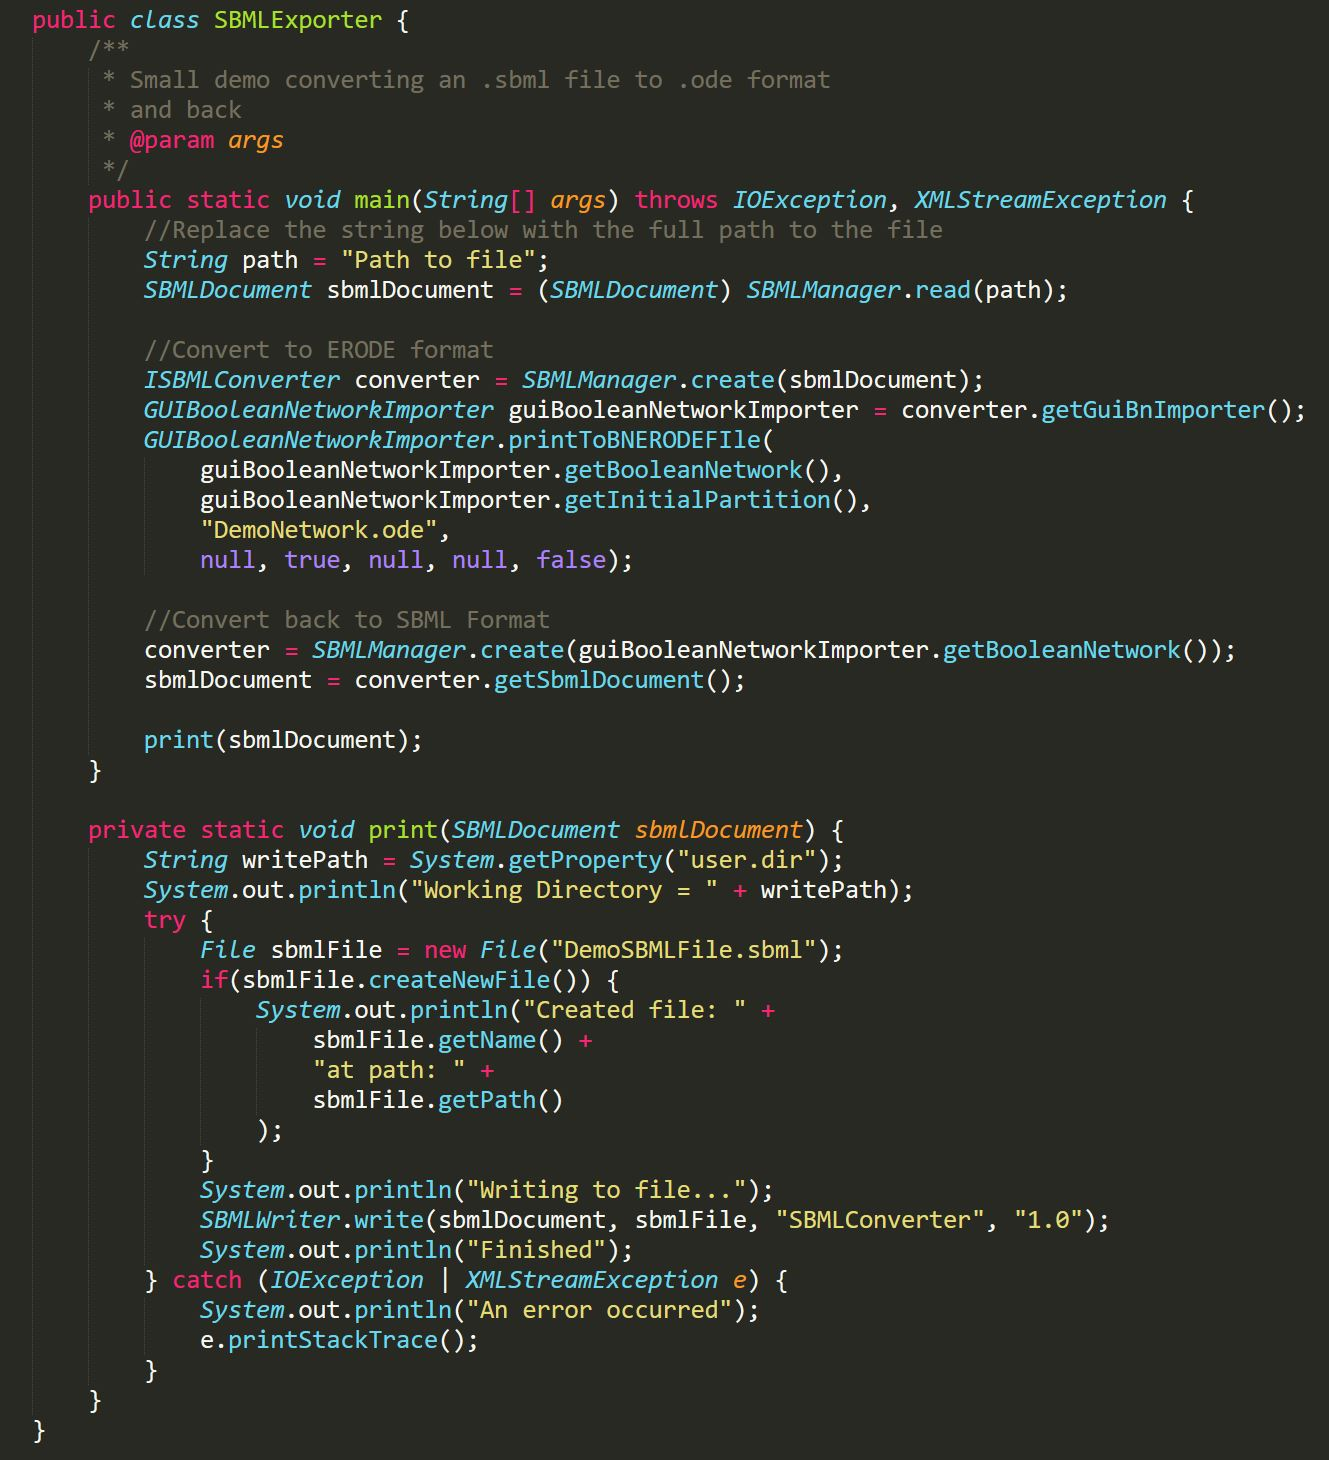
\includegraphics[scale=0.47]{Sections/Images/SBMLExporter.JPG}
    \caption{The demo program}
    \label{fig:demo}
\end{figure}

The second segment uses, the \emph{SBMLDocument} to execute the conversion to ERODE format. The conversion is executed by initialising the \emph{SBMLConverter} using the \emph{SBMLManager}'s \texttt{create()}-method. Once the conversion is complete, the \emph{GUIBooleanNetworkImporter} can be retrieved from the converter. This object contains the network model in ERODE format. ERODE's model representation is then printed to the \emph{DemoNetwork.ode}-file using ERODE's \texttt{printToBNERODEFIle()}-method. This results in the following network in \\
ERODE-format:
\pagebreak
\begin{lstlisting}[language=ERODE, caption=The ERODE formatted network]
begin Boolean network DemoNetwork
 begin init
  S_1
  S_2
  S_3
 end init
begin update functions
  S_1 = (S_2 XOR S_3)
  S_2 = ((S_1 = true)&(S_3 != true))
  S_3 = (S_1 -> (S_2 = true))
end update functions

end Boolean network
\end{lstlisting}

In the last segment of the program shown in figure \ref{fig:demo}, the converts the ERODE representation back to SBML-qual. Just like in the conversion to ERODE format, a new converter is initialized using the \emph{SBMLManager}'s \\
\texttt{create()}-method. This time however, it is given ERODE's data representation instead. Once the conversion is finished, the SBML representation is retrieved by calling the \emph{getSbmlDocument()}-method. The file is then printed to the \emph{DemoSBMLFile}.
When comparing the original input file with the newly generated file, using a file comparison tool, it can be seen that the contents of the file are identical. 
\clearpage
\chapter{Future Steps}
Considering the current state of the converter and the functionality it provides, there are a few things that could be added to the converter with further development. Suggestions for how some of these features can be implemented, can be found in the appendix.

For one, the current converter is currently unable to support multi-valued networks. However, to add the support of MNs, it would require ERODE to be extended to support them first. It should also be taken into account that such an extension can turn into very big task, since there is a larger set of network-operations that can be performed on networks in the multi-valued domain. For example, the multi-valued representation of SBML also supports the consumption of transition inputs, and production of outputs. This means, that inputs to a transition can be reduced during a transition and outputs increased, instead of overwritten.

Apart from that, there are also a series of small optimisation and extensions that can be done, that do not require ERODE to be updated. For example, algorithms that minimize the network representation could be added. This could include an update function analysis that joins output species in the same transition, given they have the same update conditions.
Another option could also be to feature algorithms that can reduce a function terms logical expression to its most compact and concise form.

A final option for further development could also be to optimize program performance by introducing concurrency. In its current state, the program runs on a single thread, since performance was of no great import. However, there are many places in the program where two independent task are performed sequentially. In these places, one could introduce concurrency to optimise the performance.
\clearpage
\chapter{Summary}
Overall, this report discusses the conversion between the SBML-qual and the ERODE format.  A converter, capable of converting back and forth between these formats, was successfully implemented.  The converter is based upon principles that render the implementation maintainable.  In other words,  one can easily extend and modify the converter if further development is needed.

To achieve this goal, several milestones, representing each stage of the project, were defined. During the first stage, the two formats haven been analyzed, to become familiar with them and obtain an overview of the conversion requirements. In the second and third stage the knowledge about the conversion requirements was then used to design and implement the converter application. Initially, a few small demo-applications were created to develop a framework for the final application. This framework was then extended into the final converter by adding new functionality iteratively. During each iteration, each new piece of functionality was tested thoroughly to ensure that the formats are converted correctly. An important part of the converter design was also to structure it in a way, that allows an integration into other host programs.

The development process was guided by a project plan to track the overall progress of the project. Additionally, weekly meetings with the project supervisors were used to discuss various aspects of the project in detail, which helped to tackle problems early and ensured progression in the project.
\clearpage
%%%%%%%%%%%%%%%%%%%%%%%%%%%%%%%%%%%%%%%%%%%%%%%%%%%%%%%

\printbibliography[heading=bibintoc,title={References}]
\cleardoublepage 
\appendix
\chapter{Appendix}
\section{Getting started with JSBML}
The most important thing to know about JSBML is that this library mostly is a literal implementation of the SBML-structures defined in the SBML specifications \cite{hucka2018systems} \cite{sbmlqual2015}. The JSBML-classes represent the structures defined in SBML, providing getter- and setter methods to populate their fields.

In figure \ref{fig:JSBMLSpecies} the steps required from reading an SBML-file to the extraction of an SBML-qual model's species are shown. After specifying the path to the SBML-file to be read, JSBML's \emph{SBMLReader} is used to read the provided file. This returns an object of type \emph{SBase}, an abstract class used for all SBML-object types, that stores meta-data about the object, such a the SBML-level and version used to represent it. To gain access to the SBML-file data representation, it need to be cast to the \emph{SBMLDocument}-type used to represent SBML-files. The \emph{Model} it contains can the be retrieved by calling the \texttt{getModel()}-method.

Model represented by one of the SBML-extensions are not represented by the \emph{Model}-class itself, but instead by a separate model-class. In case of SBML-qual, this is the \emph{QualModelPlugin-class}, which can be retrieve from the main \emph{Model} by calling the \texttt{getExtension()}-method using "qual" as an key to the extension map. In the last step of the figure, the species are then retrieved using the appropriate getter-method.

Retrieving SBML-transitions an the structures contained within, works in the same manner as with species and the other SBML-structures, which is why these are not included as a demo in this report. However, the \emph{JSBMLReadingDemo}-class in the \emph{sbml.demos} package in the repository contains a full demo of the code used to read the various SBML structures required by the converter.

\begin{figure}[H]
    \centering
    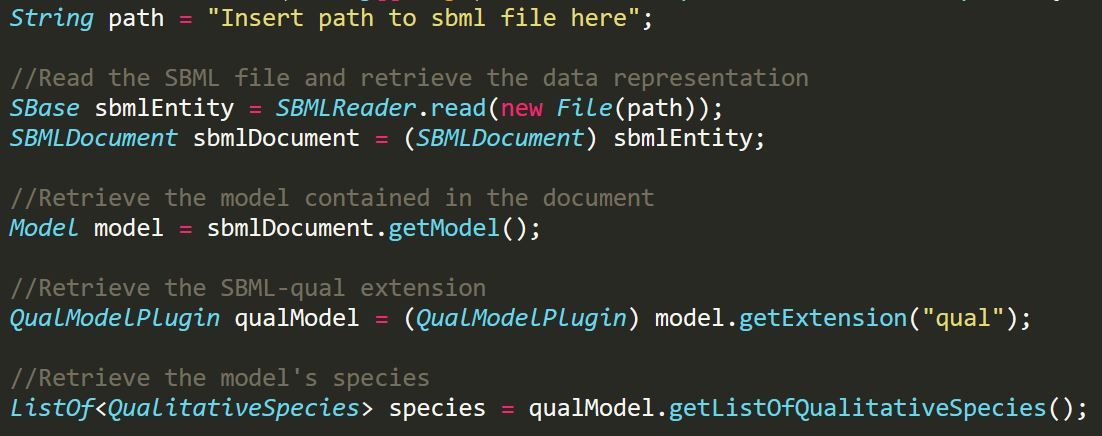
\includegraphics[scale=0.60]{Sections/Images/JSBMLSpecies.JPG}
    \caption{Species retrieval using JSBML}
    \label{fig:JSBMLSpecies}
\end{figure}

When creating object to represent SBML-structures is very important to use a consistent SBML-level and version for all object in a model representation, as JSBML will complain and throw exceptions otherwise. While almost all SBML-structures have default constructors that allow their creation without specifying level and version, it is a good idea to specify them anyway, as unset version also can cause several problems. In the converter's implementation this problem has been solved by adding a \emph{configuration}-package, which is used to set SBML-level and version for the entire converter.

In figure \ref{fig:JSBMLCreation}, it is shown how to create a small (and empty) SBML-model with an SBML-qual extension. Using either \emph{set}- or \emph{add}-methods, the various structures are added to their parents. When dealing with instances of the \emph{ListOf<>}-structure it is important to the parent of those lists to be the \emph{Model}, they are contained in. If this is not done, JSBML will not recognize these lists as part of the model and throw an exception. 

\begin{figure}[H]
    \centering
    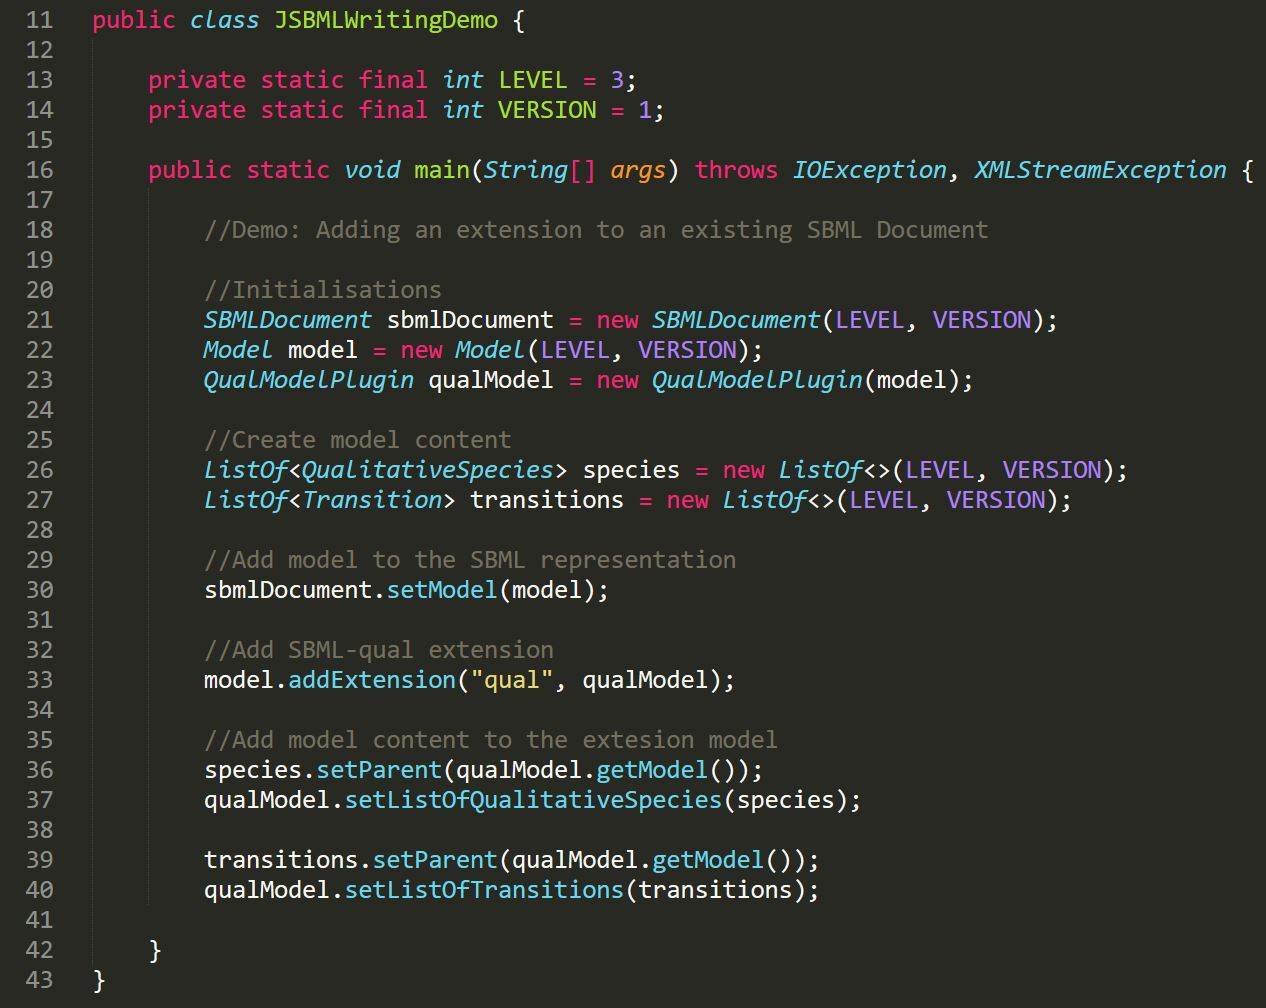
\includegraphics[scale=0.50]{Sections/Images/JSBMLCreation.JPG}
    \caption{SBML model generation using JSBML}
    \label{fig:JSBMLCreation}
\end{figure}

When dealing with the JSBML-functionality used in the converter, the last important part is to know how to create the logical expressions in the \emph{FunctionTerm}-structures used by SBML. For this, the \emph{ASTNode}-class is used, which represents the MathML-elements of an SBML-file.

 \ref{fig:ASTNode} shows the most important ways to construct \emph{ASTNodes} in this converter. Depending on what input is given to the constructor, the \emph{ASTNode} will represent a different element. As shown in the figure, variables can be create by providing the variable name in form of a string. Integer constants on the other hand are created by providing an integer value. To create other types, such as Boolean constants and operator, the \emph{ASTNode}-class also provides the \emph{Type}-enum, which defines all operators and special constants \emph{ASTNodes} can represent. The other figure (\ref{fig:ASTNode}) shows how to initialise and retrieve data from an AST consisting of \emph{ASTNode}-objects.

\begin{figure}[H]
    \centering
    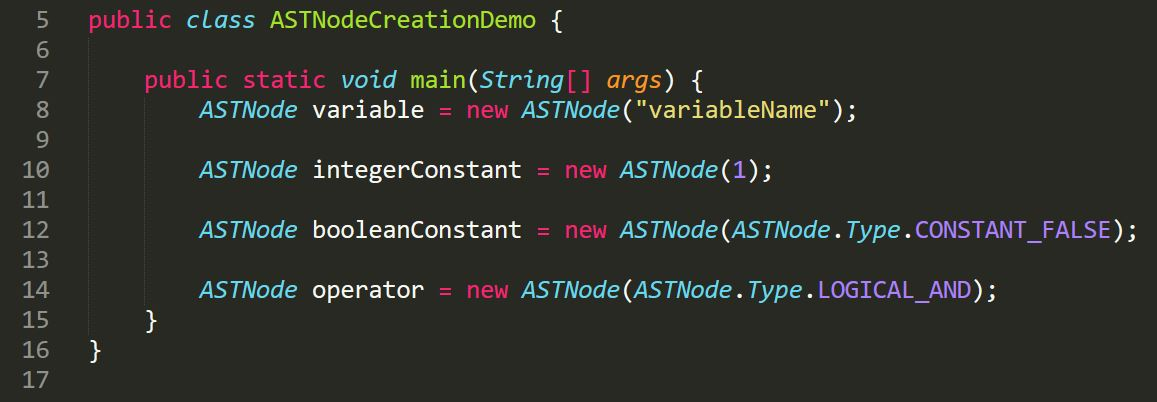
\includegraphics[scale=0.55]{Sections/Images/ASTNodes.JPG}
    \caption{Examples of ASTNodes representing elements of an AST}
    \label{fig:ASTNode}
\end{figure}

\begin{figure}[H]
    \centering
    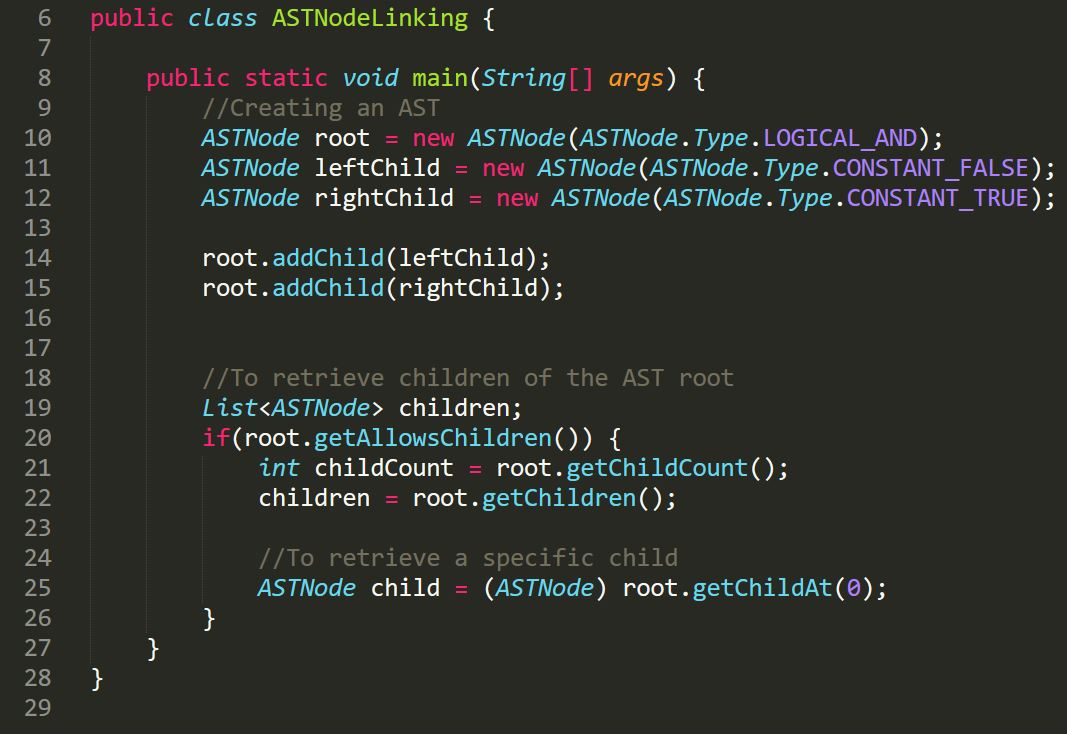
\includegraphics[scale=0.6]{Sections/Images/ASTLinking.JPG}
    \caption{Example of an AST initialisation and data retrieval from it}
    \label{fig:ASTLinking}
\end{figure}

\section{Extending the converter to support MNs}
To add support for multi-valued models in the converter only requires minor changes to the existing functionality. In total only four different methods need to be extended or modified.
Before explaining the required changes, it needs to be mentioned that the classes used to represent integer-values in ERODE, \textbf{must implement} the \emph{IUpdateFunction}-interface for this modification to work. Should this not be the case, the node conversion module in the \emph{sbml.conversion.nodes} package would need to be replaced by a different module that also implements the \emph{INodeConverter}-interface.

To extend the converter using the existing modules, the first method that needs to be modified, is the \texttt{create()}-method in the \emph{NodeManager}-class shown in figure \ref{fig:MNCreate}. This method analyzes the given update function element from ERODE's AST to analyze its type. Depending on its type, it then calls the corresponding manager to continue the converter initialisation. Since the missing update function type is a type representing integers, this is part of the \emph{ValueASTConverter}'s responsibilities.

The simplest way to modifiy is method is to move the \\
\texttt{return ValueASTConverter...} statement to the default case, replacing the current exception. Once that is done the \emph{REFERENCE},\emph{TRUE} and \emph{FALSE} cases can be removed. Since the exception in the default case currently only serves the purpose of catching the new update function type(s), once ERODE is extended it will no longer be needed.

\begin{figure}[H]
    \centering
    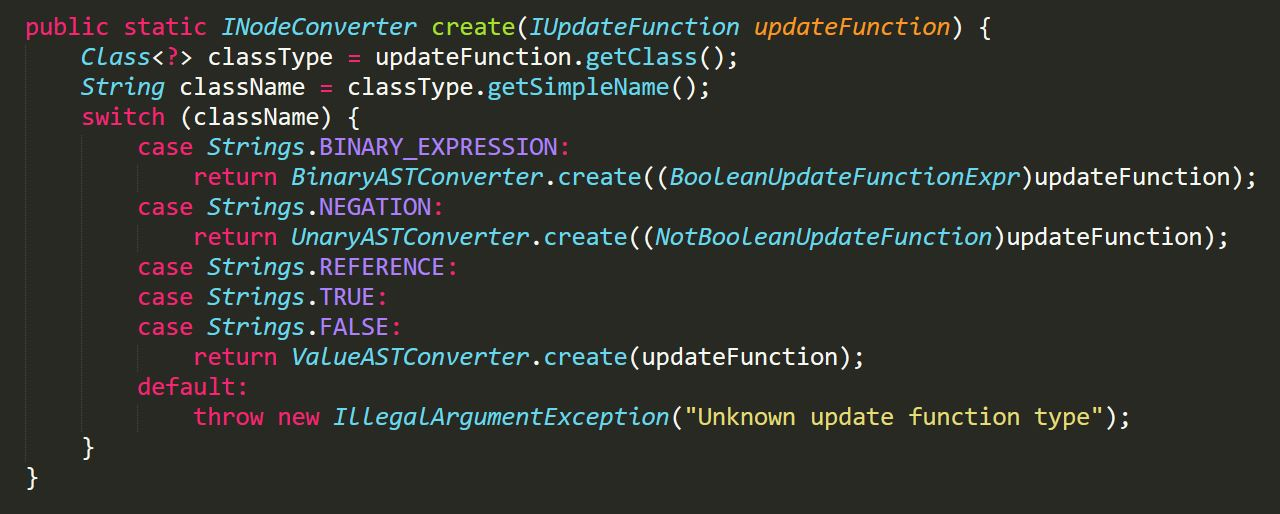
\includegraphics[scale=0.5]{Sections/Images/MNCreate.JPG}
    \caption{The \texttt{create()}-method used when converting to SBML}
    \label{fig:MNCreate}
\end{figure}

The next method to be changed, is the \emph{convert()}-method in the \emph{ValueWriter}-class. This method simply requires an additional case, to take the new update function type into account. The \emph{currentNode} for the new case should be set to the result of the \emph{element.constant()}-call.

\begin{figure}[H]
    \centering
    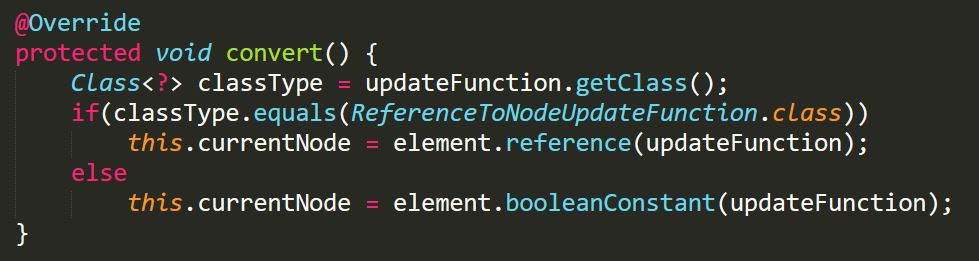
\includegraphics[scale=0.5]{Sections/Images/ValueWriterConvert.JPG}
    \caption{The \texttt{convert()}-method of the \emph{ValueWriter}-class}
    \label{fig:WriterConvert}
\end{figure}

Once these steps have been performed, the actual conversion step for the integer representations need to be implemented in the \emph{SBMLElement}-class. This class currently contains an unused method, called \texttt{constant()}, taking an \emph{IUpdateFunction}-instance as input and returns an \emph{ASTNode}, using the \emph{ASTNodeBuilder}.
The current method body, can be replaced entirely, since this method will take integer representations as input and not Boolean constants. The method body would then simply require some way of reading the \emph{IUpdateFunction}'s integer value and pass it to the \emph{ASTNodeBuilder}'s \texttt{integer()}-method, which creates integer constants.

\begin{figure}[H]
    \centering
    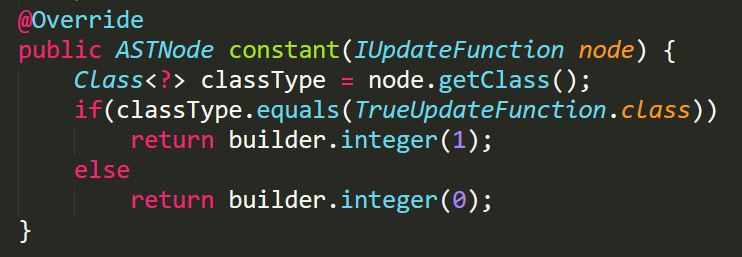
\includegraphics[scale=0.5]{Sections/Images/ConstantMethod.JPG}
    \caption{The current \texttt{constant()}-method in the \emph{SBMLElement}-class}
    \label{fig:SBMLconstant}
\end{figure}

Finally, the \texttt{constant()}-method, implemented by the \emph{ERODEElement}, also requires adjustment, since it currently translates SBML-integers to ERODE-booleans. The new version should return ERODE's integer-representation instead.

\begin{figure}[H]
    \centering
    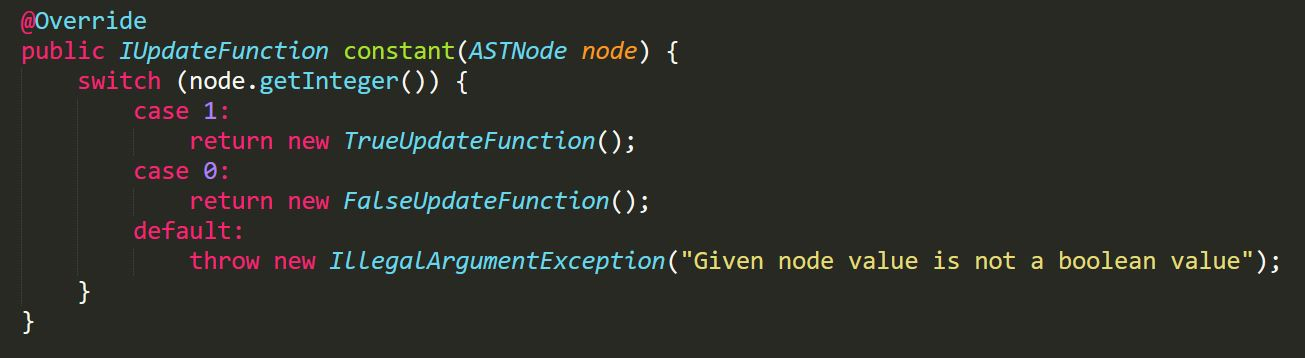
\includegraphics[scale=0.5]{Sections/Images/ERODEconstant.JPG}
    \caption{The current \texttt{constant()}-method in the \emph{ERODEElement}-class}
    \label{fig:ERODEconstant}
\end{figure}
\cleartoleftpage
\newgeometry{left=28mm,right=14mm,top=42mm,bottom=14mm}
\thispagestyle{empty}
\pagecolor{frontbackcolor}
\color{white}

\vspace*{\fill}



\begin{tabular}{@{}l}
    Technical \\ 
    University of \\ 
    Denmark \\
    \\
    \addressI \\
    \addressII \\
    Tlf. 4525 1700 \\
    \\
    \url{\departmentwebsite}
\end{tabular}



\end{document}